\documentclass[11pt,a4paper]{article}

\usepackage[utf8]{inputenc}
\usepackage[english]{babel}
\usepackage{amsmath}
\usepackage{amsthm}
\usepackage{amssymb}
\usepackage{hyperref}
\usepackage{url}
\usepackage{mathtools}
\usepackage{tikz}
\usepackage{array}
\usepackage{pifont}
\usepackage{makecell}
\usepackage{csquotes}
\usepackage{pdflscape}
\usepackage{tabularx}
\usepackage{geometry}
\usepackage[graphicx]{realboxes}


\newcommand{\cmark}{\ding{51}}
\newcommand{\xmark}{\ding{55}}

\usetikzlibrary{arrows}
\hypersetup{
    colorlinks=true,
    linkcolor=blue,
    filecolor=magenta,      
    urlcolor=blue,
    citecolor=blue,
    pdftitle={Overleaf Example},
    }
\usepackage{listings}
\usepackage{xcolor}
\definecolor{delim}{RGB}{20,105,176}
\definecolor{numb}{RGB}{106, 109, 32}
\definecolor{string}{rgb}{0.64,0.08,0.08}
\definecolor{comment}{RGB}{123,188,123}
\definecolor{greencomment}{RGB}{0,128,0} % Define the green color for comments

\lstdefinelanguage{json}{
    numbers=left,
    numberstyle=\small,
    frame=single,
    rulecolor=\color{black},
    showspaces=false,
    showtabs=false,
    breaklines=true,
    postbreak=\raisebox{0ex}[0ex][0ex]{\ensuremath{\color{gray}\hookrightarrow\space}},
    breakatwhitespace=true,
    basicstyle=\small,
    upquote=true,
    morestring=[b]",
    stringstyle=\color{string},
    literate=
     *{0}{{{\color{numb}0}}}{1}
      {1}{{{\color{numb}1}}}{1}
      {2}{{{\color{numb}2}}}{1}
      {3}{{{\color{numb}3}}}{1}
      {4}{{{\color{numb}4}}}{1}
      {5}{{{\color{numb}5}}}{1}
      {6}{{{\color{numb}6}}}{1}
      {7}{{{\color{numb}7}}}{1}
      {8}{{{\color{numb}8}}}{1}
      {9}{{{\color{numb}9}}}{1}
      {\{}{{{\color{delim}{\{}}}}{1}
      {\}}{{{\color{delim}{\}}}}}{1}
      {[}{{{\color{delim}{[}}}}{1}
      {]}{{{\color{delim}{]}}}}{1},
      morecomment=[l]{\#}, % Define the '#' character as the start of a comment
      morecomment=[s]{\#}{\ }, % Define the end of the comment
      commentstyle=\color{greencomment}, % Set the color for the '#' and the following word
}

\usepackage{graphicx}
\graphicspath{{./images/}}


\newcounter{Figcount}
\newcounter{tempFigure}

\newenvironment{TableCaption}{%
    \renewcommand{\figurename}{Table}
    \setcounter{tempFigure}{\thefigure}
    \setcounter{figure}{\theFigcount}
    }{%
    \setcounter{figure}{\thetempFigure}
    \stepcounter{Figcount}
    }


\numberwithin{equation}{section}
\newtheorem{definition}{Definition}[section]
\newtheorem{example}{Example}[section]
\newtheorem{satz}[definition]{Satz}
\newtheorem{lemma}[definition]{Lemma}
\newtheorem{fact}[definition]{Fact}
\title{Analysis of Conflicts and Dependencies between User Stories\\[0.5em] \large{Independent Scientific Work Computer Science \\[0.5em]} }

\author{Amir Rabieyan Nejad}

\date{\today}

\begin{document}

\maketitle
\begin{abstract}
In this scholarly paper, we expound upon an extensive assortment of techniques and tools that traverse diverse domains. These domains encompass agile software development, with a distinct emphasis on backlog management for the acknowledgment of user stories and their associated quality criteria. Furthermore, we delve into the realm of natural language processing (NLP) and its intricate interplay with computational lexicon resources, which is pivotal for tasks related to natural language comprehension. Additionally, we explore techniques of extracting domain models from textual requirements, which are instrumental in applying graph transformation rules and in discerning conflicts and dependencies among user stories.

The principal objective of our scholarly pursuit is to conduct a comparative analysis of these techniques and tools within each domain. Our intention is to harness this analysis for future endeavors, aiming to establish a meticulously structured workflow. This framework holds the promise of expediting the automated detection of conflicts and dependencies inherent within user stories expressed in natural language.

\end{abstract}
\newpage
\tableofcontents
\newpage



\section{Introduction}
User stories, the fundamental building blocks of software development, serve as concise and testable descriptions of a program's functionality. Within the dynamic framework of agile development, these user stories are typically composed informally, using plain text, and they are maintained in the product backlog, which acts as a repository for prioritizing and tracking development tasks.

Behaviour Driven Development (BDD), a specialized approach within the realm of agile software development, places a strong emphasis on the iterative implementation of user stories. The sequencing of user stories in BDD is a pivotal aspect of the methodology. The right sequence not only impacts the efficiency of development but also the overall success of the project. By prioritizing and sequencing user stories effectively, development teams can deliver incremental value to users, respond to changing requirements, and ensure that the most critical functionality is addressed first.

User stories often exhibit dependencies on one another, leading to potential conflicts in which one user story necessitates the deletion of a component vital to the successful execution of another user story, or one user story may introduce an element that contravenes and thus prohibits the realization of another user story. To minimize the occurrence of conflicts, teams should systematically identify and document dependencies between user stories within their backlog. Agile methodologies, such as Scrum, promote cross-functional collaboration and daily stand-up meetings as mechanisms for promptly addressing and mitigating dependencies and conflicts. However, this approach can be time and resource-intensive. In instances where the backlog is extensive, the recognition of existing conflicts between user stories can become a complex endeavour.

To achieve the automation of conflict and dependency resolution within the scope of user stories associated with a single backlog, it is imperative that we establish a well-structured workflow. This workflow should encompass a collection of techniques and tools derived from various domains. 

In this research paper, we embark on a comprehensive exploration of cutting-edge techniques and methodologies in the realm of natural language processing (NLP) and computational lexicon resources, a symbiotic relationship that holds pivotal significance for tasks pertaining to natural language comprehension. Furthermore, we embark on an exploration of techniques which extracting domain models from textual requirements, pivotal disciplines enabling the application of graph transformation rules and the discernment of conflicts and dependencies among user stories.

Section \ref{usq} introduces fundamental concepts, providing the necessary background information about \emph{user story} and \emph{backlog}. Additionally, we delve into the techniques employed in the User Story Quality and compare these techniques with each other. Moving forward to Section \ref{dmodel}, we conduct a comparative analysis of various approaches extracting domain models from textual requirements, with a specific focus on efficient backlog management geared towards the recognition of user stories. Section \ref{nlp} is dedicated to a comparative analysis of several computational lexical resource techniques. The aim is to identify the most appropriate verb lexicon for the categorization of verbs found within user stories into three distinct categories, thereby facilitating the formulation of precise transformation rules. Section \ref{gts} centers on the comparison of methods for generating graph transformation rules. Finally, section \ref{conclusion} conclude the paper. 

%\section{Role of User Stories and Backlogs in Agile Development}\label{us}
The agile software development paradigm broke the wall that classically existed between the development team and end-users. Thanks to the involvement of a Product Owner (PO) who acts as a proxy to end-users for the team, the product backlog \cite{sedano2019product} became a first-class citizen during the product development. Furthermore, thanks to a set of user stories expressing features to be implemented in the product in order to deliver value to end-users, the development teams were empowered to think in terms of added value when planning their subsequent developments. The product is then developed iteration by iteration, incrementally. Each iteration selects a subset of the stories, maintaining a link between the developers and the end-users\cite{mosser2022modelling}. 

\emph{Ordinarily, User Stories typically exhibit interdependencies, wherein the order of their implementation becomes a critical consideration. This circumstance raises the question of how one may discern and identify the relationships that exist between the User Stories.}

Sedano et al. posited that a “product backlog is an informal model of the work to be done” \cite{sedano2019product}. A backlog implements a shared mental model over practitioners working on a given product, acting as a boundary artifact between stakeholders. This model is voluntarily kept informal to support rapid prototyping and brainstorming sessions. Classically, backlogs are stored in project management systems, such as \footnote{\href{https://www.atlassian.com/en/software/jira}{Jira Software}} Jira. These tools store user stories as tickets, where stakeholders write text as natural language. Meta-data (e.g., architecture components, severity, quality attribute) can also be attached to the stories. However, there is no formal language to express stories or model backlogs from a state of practice point of view.

A user story is a brief, semi-structured sentence and informal description of some aspect of a software system that illustrates requirements from the user’s perspective \cite{raharjana2021user}. Large, vague stories are called epics. While user stories vary widely between organizations, most observed stories included a motivation and acceptance criteria. The brief motivation statement followed the pattern:  As a  \textless\emph{user}\textgreater\ I want to \textless\emph{action}\textgreater\ so that \textless\emph{value}\textgreater. This is sometimes called the Connextra template. The acceptance criteria followed the pattern: Given \textless\emph{context}\textgreater, when \textless\emph{condition}\textgreater \  then \textless\emph{action}\textgreater. This is sometimes called Gherkin syntax \cite{wynne2017cucumber}. It consists of three aspects, namely aspects of who, what and why. The aspect of “who” refers to the system user or actor, “what” refers to the actor’s desire, and “why” refers to the reason (optional in the user story) \cite{raharjana2021user}.

The user story components consist of the following elements \cite{wautelet2017user} : \emph{Role}: abstract behavior of actors in the system context; the aspect of who representation. \emph{Goal}: a condition or a circumstance desired by stakeholders or actors. Task: specific things that must be done to achieve goals. \emph{Capability}: the ability of actors to achieve goals based on certain conditions and events.

\section{User Story Quality Analysis Techniques}\label{usq}
In this section, we embark on an exposition of methodologies with the specific objective of refining the precision of User Stories measurement. First, in subsection \ref{us} the role of USs and backlogs in agile development will be discussed. Additionally, the most common pattern of US will be introduced.

From subsection \ref{invest} our focus centers on the exploration of established techniques to address the query regarding the existence of criteria for the management and identification of conflicts and dependencies among User Stories. Furthermore, our attention is directed towards the criteria they employ, a pivotal factor in ensuring the creation of well-structured and standardized User Stories. Subsequent to this exploration, we undertake a comprehensive comparative analysis of these methodologies to ascertain the approach that best aligns with our particular contextual requirements.
\subsection{Role of User Stories and Backlogs in Agile Development} \label{us}
The agile software development paradigm broke the wall that classically existed between the development team and end-users. Thanks to the involvement of a Product Owner (PO) who acts as a proxy to end-users for the team, the product backlog \cite{sedano2019product} became a first-class citizen during the product development. Furthermore, thanks to a set of user stories expressing features to be implemented in the product in order to deliver value to end-users, the development teams were empowered to think in terms of added value when planning their subsequent developments. The product is then developed iteration by iteration, incrementally. Each iteration selects a subset of the stories, maintaining a link between the developers and the end-users\cite{mosser2022modelling}. 

\textbf{\emph{Ordinarily, User Stories typically exhibit interdependencies, wherein the order of their implementation becomes a critical consideration. This circumstance raises the question of how one may discern and identify the relationships that exist between the User Stories.}}

Sedano et al. posited that a “product backlog is an informal model of the work to be done” \cite{sedano2019product}. A backlog implements a shared mental model over practitioners working on a given product, acting as a boundary artifact between stakeholders. This model is voluntarily kept informal to support rapid prototyping and brainstorming sessions. Classically, backlogs are stored in project management systems, such as \footnote{\href{https://www.atlassian.com/en/software/jira}{Jira Software}} Jira . These tools stores user stories as tickets, where stakeholders write text as natural language. Meta-data (e.g., architecture components, severity, quality attribute) can also be attached to the stories. However, there is no formal language to express stories or model backlogs from a state of practice point of view.

A user story is a brief, semi-structured sentence and informal description of some aspect of a software system that illustrates requirements from the user’s perspective \cite{raharjana2021user}. Large, vague stories are called epics. While user stories vary widely between organizations, most observed stories included a motivation and acceptance criteria. The brief motivation statement followed the pattern:  As a  \textless\emph{user}\textgreater\ I want to \textless\emph{action}\textgreater\ so that \textless\emph{value}\textgreater. This is sometimes called the Connextra template . The acceptance criteria followed the pattern: Given \textless\emph{context}\textgreater, when \textless\emph{condition}\textgreater \  then \textless\emph{action}\textgreater. This is sometimes called Gherkin syntax \cite{wynne2017cucumber}. It consists of three aspects, namely aspects of who, what and why. the aspect of “who” refers to the system user or actor, “what” refers to the actor’s desire, and “why” refers to the reason (optional in the user story) \cite{raharjana2021user}.

The user story components consist of the following elements \cite{wautelet2017user} : \emph{Role}: abstract behavior of actors in the system context; the aspect of who representation. \emph{Goal}: a condition or a circumstance desired by stakeholders or actors. Task: specific things that must be done to achieve goals. \emph{Capability}: the ability of actors to achieve goals based on certain conditions and events.
\subsection{Improving User Story using INVEST Criteria} \label{invest}
In Agile software development, effective requirement management is crucial for delivering valuable and high-quality software. The INVEST criteria serve as a set of guiding principles that help teams assess and shape their user stories and requirements to meet the demands of Agile development. Each letter in the acronym INVEST represents a fundamental attribute that a requirement should possess to maximize its effectiveness within an Agile context.

These criteria were introduced to ensure that Agile teams create requirements that are not only clear and actionable but also adaptable to changing circumstances. The goal is to promote flexibility, collaboration, and a relentless focus on delivering value to the end-users or stakeholders \cite{buglione2013improving}.

In the following, we will examine the individual INVEST criteria in depth, with a focus on explaining their importance and their pragmatic application in the context of Agile Requirement Engineering \cite{cohn2004user}. \\ 
\textbf{Independent} \\ 
Independent emphasize the avoidance of interdependencies between user stories or requirements. This principle underscores the importance of ensuring that each requirement operates autonomously, without relying on the completion of other related requirements. The presence of dependencies among requirements can introduce complexities in the prioritization and planning phases of Agile development. Such dependencies may necessitate a specific order of implementation, hindering the team's ability to adapt to changing priorities and potentially causing delays in project delivery. \\ 
\textbf{Negotiable}\\ 
 USs (User Stories) should not be construed as rigid, contractual obligations or exhaustive lists of requirements that the software must adhere to. Instead, they are viewed as dynamic entities, open to ongoing discussion and refinement.

US are not meant to encapsulate every conceivable detail at the outset. The inclusion of excessive details can create a deceptive illusion of precision or completeness, potentially stifling the need for continued dialogue and collaboration. 

An essential attribute of negotiable USs is their inherent flexibility. It is crucial to avoid treating User Stories as contractual obligations, as this can lead to a rigid mindset where estimates and commitments are made with the same level of inflexibility as a traditional contract. Instead, Agile teams should recognize the negotiable nature of USs and remain open to adapting them as circumstances warrant. \\ 
\textbf{Valuable}\\ 
The criterion of Value underscores that US must possess inherent worth and significance. A US should be designed in such a way that it delivers tangible value to either the end-users or the stakeholders. The value encapsulated within a US can manifest in various forms, such as improved user experiences, enhanced functionality, increased efficiency, or meeting specific business objectives.

Agile teams should prioritize and select USs that offer real, quantifiable value, as this ensures that the development effort is consistently directed toward outcomes that align with the project's overarching goals and objectives.

The concept of Value serves as a guiding principle that encourages Agile teams to continuously assess and prioritize USs based on their potential to contribute positively to the project's success, ultimately enhancing the overall quality and impact of the software being developed.\\ 
\textbf{Estimable}\\ 
An essential condition for a US to be deemed Estimable is that it must be sufficiently well-defined and clear. Ambiguity or lack of clarity within a US can render it inestimable, meaning that the development team cannot provide a reliable estimate of the effort required for implementation.

Estimable USs facilitate the planning process by enabling the team to make informed decisions about the allocation of resources, timeframes, and priorities. Clear and concise USs ensure that the estimation process is based on a solid foundation of understanding, leading to more accurate project planning and execution. \\  
\textbf{Small}\\ 
The attribute of smallness is a pivotal aspect of the INVEST criteria for USs. It pertains to the size and granularity of individual USs. Large stories, present several challenges in Agile development. They tend to be intricate and challenging to estimate accurately. 

A Complex Story refers to a US that is inherently large and resistant to disaggregation into smaller, more granular stories. Complex stories are a source of concern in Agile development because they can hinder effective planning and may require special consideration and strategies to address. Additionally, they pose difficulties in terms of fitting into single iterations or sprints.\\ 
\textbf{Testable}\\ 
The testable attribute signifies that USs should be structured in a manner that allows for the clear demonstration of whether they meet the customer's expectations. The verification of meeting these expectations is typically accomplished through testing.

An overarching goal in Agile development is to maximize the efficiency and effectiveness of testing processes. To achieve this, Agile teams strive for a high degree of test automation, with a target of attaining a test automation rate exceeding 90\%.

Test automation plays a pivotal role in Agile development by enabling rapid and repeatable testing of software features. Automated tests ensure that the software remains consistent with the desired functionality outlined in the US, thereby reducing the risk of regressions and defects.

INVEST grid in table \ref{tb:invest} can be used as a template when the customer and provider meet to evaluate a US \cite{buglione2013improving}.

The INVEST criteria serve as fundamental guidelines that are partially incorporated into the definition of many existing quality frameworks and requirement development tools in Agile methodologies.\\ \\ 


\newgeometry{margin=2.5cm}

\thispagestyle{empty}


\begin{figure}

\begingroup

\footnotesize
\Rotatebox{90}{%

\begin{tabularx}{25cm}{c  X  X  X  X  X}
 INVEST & \multicolumn{1}{c}{Description} & \multicolumn{1}{c}{0} & \multicolumn{1}{c}{1} & \multicolumn{1}{c}{2} & \multicolumn{1}{c}{3} \\
  &  & \multicolumn{1}{c}{Poor/Absent} & \multicolumn{1}{c}{Fair} & \multicolumn{1}{c}{Good} & \multicolumn{1}{c}{Excellent} \\
\hline
\hline
\\
 I – Independent & User Stories should be as independent as possible & The start of construction of a US is tied to the completion of at least one other US & The completion of a US hinders the start of construction of at least one other US  & The US can contain any constraint, but its release can be constrained by the completion of at least one other US  & The US is fully independent, and it can be realized and released with any constraint \\
 \\
 N – Negotiable & User Stories should be "open”, reporting any relevant details as much as possible & The US contains enough detail to be a technical specification (Design phase), leaving no room to negotiate any element & The US is written with enough detail to be a functional specification (Analysis phase), leaving no room to negotiate any element & The US is written with informative content defining a User Requirement in a consolidated manner, yet shared between Customer and Provider  & The US is written with the informative content typical of a high-level need, allowing feedback between customer and provider \\
\\
 V – Valuable & User Stories should provide value to end users in terms of the solution & The functional part (F) of the US does not contain all the functionalities requested by the customer & The functional (F) part of the US expresses mostly qualitative (Q) and technical (T) requirements about the system, and needs to be more developed in terms of functional requirements & The functional (F) part of the US expresses mostly the functional requirements requested by the Customer, but also includes qualitative (Q) and technical (T) requirements & The functional (F) part of the US correctly expresses only the functional requirements requested by the customer \\

 \\
 E – Estimable & Each User Story must be able to be estimated in terms of relative size and effort & The US shows only its functional (F) part, filled in by the customer, but without sufficient detail to allow the provider to fill in the Q/T parts & The US shows only its functional (F) part, filled in by the customer, but validated with the provider  & The US has been completed by the provider with respect to Q/T issues, but still needs to be validated jointly with the customer & All the useful parts of the US (F/Q/T) are shown, allowing the effort need to size and estimate it, and validated by both parts \\

 \\
 S – Small & Each User Story should be sufficiently granular, and not defined at too high a level & The US is very large, and cannot be completed within a Sprint & The US is very large, and can be completed within a Sprint, but cannot accommodate the creation/delivery of other US & The size of the US is such that it can be completed within a Sprint, jointly with other US, but it is too small to create overhead about the Testing phase  & The size of the US is such that it can be completed within a Sprint, jointly with other US, ensuring an appropriate balance between development and testing activities \\

 \\
 T – Testable & Each User Story must be formulated in an effort to stress useful details for creating tests & The US does not include tips about Acceptance Tests & The US includes a formal indication of Acceptance Tests, but yet to be completed & The US includes an indication of Acceptance Tests which are complete, but yet to be validated & The US includes an indication of completed and validated Acceptance Tests \\
 \\
 \hline

\end{tabularx}

}%
\begin{TableCaption}
\caption{INVEST Grid \cite{buglione2013improving}}\label{tb:invest}
\end{TableCaption}
\endgroup
\end{figure}
\restoregeometry
\subsection{A Quality Framework} \label{usq_2}
In this section we introduce the quality framework which use traditional requirement known as the Software Product Certification Model (SPCM)\cite{heck2010software} to establish quality criteria for agile requirements. SPCM is based on extensive literature research for traditional up-front requirements engineering. 

In order to certification two types of input are required: (1) one or more software artifacts and (2) on or more properties of these artefacts that are to be certified. The SPCM divides a software artifact into six Product Areas, namely the \emph{Context Description}, which describes the environment of the system, the \emph{User Requirement}, the \emph{High-Level Design}, the \emph{Detailed Design}, the \emph{Implementation} and \emph{Test}. Next to the division, the SPCM defines specific certification criteria for each area \cite{heck2010software}. The properties of these artifacts which Heck et al. have denoted as \enquote{Conformance Properties}, can fall into one of the following categories:

\begin{itemize}
\item Consistency: do the different (parts of) software artifacts conform to each other?
\item Functional: does input to the system produce the expected output?
\item Behavioral: does the system meet general safety and progress properties like absence of deadlocks or are constraints on the specific states of the system met?
\item Quality: do the artifacts fulfill nonfunctional requirements in the areas of for example performance, security, and usability?
\item	Compliance: do the artifacts conform to standards, guidelines, or legislation?

\end{itemize}

Based on the SPCM they define three overall criteria for agile requirements \cite{heck2014quality}: 
\textbf{Completeness}\\ 
All elements of the agile requirement should be present. Three levels have considered: \emph{basic} elements, \emph{required} elements, \emph{optional }elements. In that way it can differentiate between elements that are absolutely mandatory for a requirement and elements that are nice to have because they increase the requirement quality. \\ 
\textbf{Uniformity}\\ 
The style and format of the agile requirements should be standardized, because this leads to less time for understanding and managing the requirements. Each time a team member is confronted with a new requirement he/she needs some time to understand the requirement and decide what to do with it. This process takes less time when the requirements format is standardized. Then all team members know where to look for what information on the requirement or how to read certain models attached to the requirement. \\ 
\textbf{Conformance}\\ 
Each element in the requirements is described in a correct and consistent way. The relations between the elements in the requirements description and with the context description are correct and consistent. They should be subject to manual verification, as: two requirements or use cases contradict each other; No requirement is ambiguous; Functional requirements specify what, not how; Each requirement is testable; Each requirement is uniquely identified; Each requirement is atomic; The glossary definitions are non-cyclic; Use case diagrams correspond to use case text; The data model diagram is in normal form.

The following criteria are explicitly delineated for USs, as depicted in figure \ref{fig:arvf}:
\begin{figure}
\center
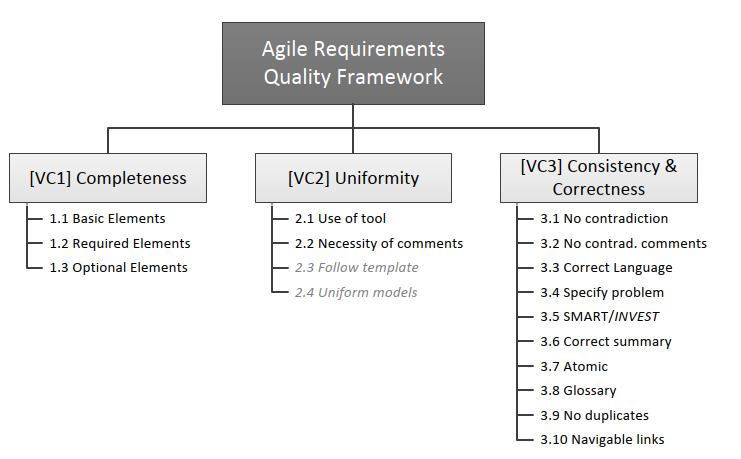
\includegraphics[width=13.03cm, height=7.76cm]{Agile_Requirements_Verification_Framework}
\caption{Agile Requirements Verification Framework \cite{heck2014quality}}\label{fig:arvf}
\end{figure}


\begin{itemize}
\item Basic Elements: Role, activity, business value (‘Who needs what why?’) instead of summary and description
\item Required Elements: acceptance criteria or acceptance tests to verify the story instead of rationale
\item Optional Elements: the team could agree to more detailed attachments to certain user stories (e.g. UML models) for higher quality
\item Stories Uniform: each user story follows the standard user voice form
\item Attachments Uniform: any modeling language used in the attachments is uniform and standardized
\end{itemize}


\subsection{QUS framework} \label{usq_3}
Lucassen et al. \cite{lucassen2016improving} represent a Quality User Story (QUS) framework, which consist of 13 quality criteria that US writers should strive to conform to. Subjected criteria determine the intrinsic quality of USs in terms of syntax, pragmatics, and semantics (Figure \ref{fig:qus_framework}; Table \ref{tb:qus}). Base on QUS, Lucassen et al. present the Automatic Quality User Story Artisan (AQUSA) software tool for assessing and enhancing US quality. Relying on NLP techniques, AQUSA detects quality defects and suggests possible remedies.

A user story should follow some pre-defined, agreed upon template chosen from the many existing ones \cite{wautelet2014unifying}. The skeleton of the template is called \emph{format} in the conceptual model, in between which the \emph{role}, \emph{means}, and optional \emph{end(s)} are interspersed to form a user story. 

Because USs are a controlled language, the QUS framework’s criteria are organize in Lindland’s categories \cite{lindland1994understanding}:

\begin{itemize}
\item\emph{ Syntactic quality}, concerning the textual structure of a US without considering its meaning;
\item \emph{Semantic quality}, concerning the relations and meaning of (parts of) the US text;
\item \emph{Pragmatic quality}, considers the audience’s subjective interpretation of the user story text aside from syntax and semantics.
\end{itemize}

First, Lucassen et al. introduced quality criteria that can be evaluated against an individual US by presenting an explanation of the criterion as well as an example US that violates the specific criterion.


\begin{figure}
\center
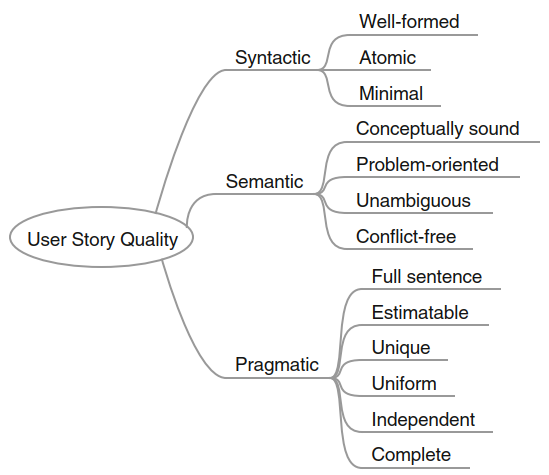
\includegraphics[width=10.03cm, height=7.76cm]{Quality_US_framework_that_define_13_criteria_for_US_quality_overview}
\caption{Agile Requirements Verification Framework \cite{lucassen2016improving}}\label{fig:qus_framework}
\end{figure}

\begin{figure}
\begingroup
\footnotesize

\begin{tabularx}{\textwidth}{l  X  c}
 \hline
 Criteria & Description & Individual/Set \\
\hline
\hline
\\
\textbf{Syntactic} \\
\\ 
Well-formed & A user story includes at least a role and a means & Individual \\
Atomic & A user story expresses a requirement for exactly one feature & Individual \\
Minimal & A user story contains nothing more than role, means, and ends & Individual \\
\\ 
 \textbf{Semantic} \\
 \\ 
Conceptually sound&The means expresses a feature and the ends expresses a rationale & Individual\\
Problem-oriented& A user story only specifies the problem, not the solution to it& Individual\\
Unambiguous&A user story avoids terms or abstractions that lead to multiple interpretations &Individual \\
Conflict-free&A user story should not be inconsistent with any other user story &Set \\
\\ 
\textbf{Pragmatic}\\
\\ 
Full sentence&A user story is a well-formed full sentence &Individual \\
Estimable&A story does not denote a coarse-grained requirement that is difficult to plan and prioritize &Individual \\
Unique&Every user story is unique, duplicates are avoided &Set \\
Uniform&All user stories in a specification employ the same template &Set \\
Independent&The user story is self-contained and has no inherent dependencies on other stories &Set \\
Complete&Implementing a set of user stories creates a feature-complete application, no steps are missing &Set \\
 \\
 \hline

\end{tabularx}
\begin{TableCaption}
\caption{Quality User Story framework that defines 13 criteria for user story quality: details \cite{lucassen2016improving}}\label{tb:qus}
\end{TableCaption}
\endgroup
\end{figure}
\textbf{Independent}\\ 
USs should not overlap in concept and should be schedule and implementable in any order. 

Complete independence may not always be achievable, the recommendation is to make any dependencies explicit and visible. Additionally, resolving certain dependencies may not be possible, and it is suggested practically approaches such as adding notes to story cards or using hyperlinks in issue trackers to make these dependencies evident. Two illustrative cases of dependencies are presented:
\begin{itemize}
\item 	\emph{Causality}: In some cases, one user story ($l_1$) must be completed before another ($l_2$) can begin. This is formalized as the predicate \enquote{$hasDep(l_1, l_2)$}, indicating that $ l_1$ causally depends on $l_2$ when specific conditions are met.
\item 	\emph{Superclasses}: USs may involve an object (\emph{e.g.}, \enquote{Content} in US \enquote{As a User, I am able to edit the content that I added to a person’s profile page}) that refers to multiple other objects in various stories, implying that the object in $l_1$ serves as a parent or superclass for the other objects.
\end{itemize}
\textbf{Well-formed}\\ 
Before it can be considered a US, the core text of the requirement needs to include a role and the expected functionality: the \emph{means}. Considering the US \enquote{I want to see an error when I cannot see recommendations after I upload an article}. It is likely that the US writer has forgotten to include the role. The story can be fixed by adding the role: \enquote{As a Member, I want to see an error when I cannot see recommendations after I upload an article.}.\\ 
\textbf{Atomic}\\ 
A user story should concern only one feature. Although common in practice, merging multiple user stories into a larger, generic one diminishes the accuracy of effort estimation\cite{liskin2014we}. For instance, the US \enquote{As a User, I am able to click a particular location from the map and thereby perform a search of landmarks associated with that latitude longitude combination} consist of two separate requirements: the act of clicking on a location and the display of associated landmarks. This US should be split into two:
\begin{itemize}
\item $US_A$: \enquote{As a User, I’m able to click a particular location from the map};
\item $US_B$: \enquote{as a User, I’m able to see landmarks associated with the latitude and longitude combination of a particular location}.
\end{itemize}
\textbf{Minimal}\\ 
User stories should contain a role, a means, and (optimally) some ends. Any additional information such as comments, descriptions of the expected behaviour, or testing hints should be left to additional notes. Consider the US \enquote{As a care professional, I want to see the registered hours of this week (split into products and activities). See: Mockup from Alice NOTE—first create the overview screen—then add validations}: Aside from a role and means, it includes a reference to an undefined mockup and a note on how to approach the implementation. The requirements engineer should move both to separate user story attributes like the description or comments, and retain only the basic text of the story: \enquote{As a care professional, I want to see the registered hours of this week.} \\ 
\textbf{Conceptually sound}\\ 
The means and end parts of a user story play a specific role. The means should capture a concrete feature, while the end expresses the rationale for that feature. Consider the US \enquote{As a User, I want to open the interactive map, so that I can see the location of landmarks}: The end is actually a dependency on another (hidden) functionality, which is required in order for the means to be realized, implying the existence of a landmark database which is not mentioned in any of the other stories. A significant additional feature that is erroneously represented as an end, but should be a means in a separate user story, for example:
\begin{itemize}
\item $US_A$: \enquote{As a User, I want to open the interactive map};
\item $US_B$: \enquote{As a User, I want to see the location of landmarks on the interactive map.}.
\end{itemize}
\textbf{Problem-oriented}\\ 
In line with the problem specification principle for RE proposed by Zave and Jackson \cite{zave1997four}, a user story should specify only the problem. If absolutely necessary, implementation hints can be included as comments or descriptions. Aside from breaking the minimal quality criteria, this US \enquote{As a care professional I want to save a reimbursement—add save button on top right (never grayed out)} includes implementation details (a solution) within the user story text. The story could be rewritten as follows: \enquote{As a care professional, I want to save a reimbursement.}. \\ 
\textbf{Unambiguous}\\ 
Ambiguity is intrinsic to natural language requirements, but the requirements engineer writing user stories has to avoid it to the extent this is possible. Not only should a user story be internally unambiguous, but it should also be clear in relationship to all other user stories. The Taxonomy of Ambiguity Types \cite{berry2004ambiguity} is a comprehensive overview of the kinds of ambiguity that can be encountered in a systematic requirements specification.

In this US \enquote{As a User, I am able to edit the content that I added to a person's profile page}, \enquote{content} is a superclass referring to audio, video, and textual media uploaded to the profile page as specified in three other, separate user stories in the real-world user story set. The requirements engineer should explicitly mention which media are editable; for example, the story can be modified as follows: \enquote{As a User, I am able to edit video, photo and audio content that I added to a person’s profile page.}. \\ 
\textbf{Full sentence}\\ 
A user story should read like a full sentence, without typos or grammatical errors. For instance, the US \enquote{Server configuration} is not expressed as a full sentence (in addition to not complying with syntactic quality). By reformulating the feature as a full sentence user story, it will automatically specify what exactly needs to be configured. For example, US \enquote{Server configuration} can be modified to \enquote{As an Administrator, I want to configure the server’s sudo-ers.} \\ 
\textbf{Estimatable}\\ 
As user stories grow in size and complexity, it becomes more difficult to accurately estimate the required effort. Therefore, each user story should not become so large that estimating and planning it with reasonable certainty becomes impossible \footnote{\href{http://xp123.com/articles/invest-in-good-stories-and-smart-tasks/. Accessed 2015-02-18}{INVEST in good stories, and SMART tasks}}. For example, the US \enquote{As a care professional I want to see my route list for next/future days, so that I can prepare myself (for example I can see at what time I should start traveling)} requests a route list so that care professionals can prepare themselves. 

While this might be just an unordered list of places to go to during a workday, it is just as likely that the feature includes ordering the routes algorithmically to minimize distance travelled and/or showing the route on a map. These many functionalities inhibit accurate estimation and call for splitting the user story into multiple user stories; for example:
\begin{itemize}
\item $US_A$: \enquote{As a Care Professional, I want to see my route list for next/future days, so that I can prepare myself};
\item $US_B$: \enquote{As a Manager, I want to upload a route list for care professionals.}.
\end{itemize}

The subsequent quality criteria pertain to a collection of USs. These quality criteria are instrumental in the assessment of the overall project specification's quality, focusing on the entirety of the project specification as opposed to the individual scrutiny of individual stories: \\ 
\textbf{Unique and Conflict-Free}\\ 
The concept of unique user stories, emphasizing the avoidance of semantic similarity or duplication within a project. For example considering $EP_a$: \enquote{as a Visitor, I am able to see a list of news items, so that I stay up to date} and $US_a$: \enquote{As a Visitor, I am able to see a list of news items, so that I stay up to date}. This situation can be improved by providing more specific stories, like:
\begin{itemize}
\item $US_{\text{a1}}$ \enquote{As a Visitor, I am able to see breaking news;}
\item $US_{\text{a2}}$ \enquote{As a Visitor, I am able to see sports news.}
\end{itemize}
Additionally, the importance of avoiding conflicts between user stories should be considered to ensure their quality. \textbf{\emph{A requirements conflict occurs when two or more requirements cause an inconsistency}} \cite{paja2013managing} \cite{robinson1989integrating}. For instance, considering story $US_b$: \enquote{As a User, I am able to edit any landmark} contradicts the requirement that a user can edit any landmark ($US_c$: \enquote{As a User, I am able to delete only the landmarks that I added}), if we assume that editing is a general term that includes deletion too. $US_b$ refers to any landmark, while  $US_c$ only those that user has added. A possible way to fix this is to change $US_b$ to: \enquote{As a User, I am able to edit the landmarks that I added.} \cite{lucassen2016improving}

%For instance, considering the stories $US_b$:\enquote{As a User, I am able to edit any landmark} and $US_c$: \enquote{As a User, I am able to delete only the landmarks that I added} and assuming that editing is a general term that includes deletion, these two user stories are contradicting. The conflict is \enquote{any landmark} versus \enquote{the landmark that I added}.  A possible way to fix this is to delete one of the user stories or explicitly excluding the deletion from $US_b$ (\emph{i.e.} \enquote{As a User, I am able to add and modify any landmark})
To detect these types of relationships, each US part needs to be compared with the parts of the other USs, using a combination of similarity measures that are either syntactic (\emph{e.g.}, Levenshtein’s distance) or semantic (\emph{e.g.}, employing an ontology to determine synonyms). When similarity exceeds a certain threshold, a human analyst is required to examine the user stories for potential conflict and/or duplication.
\begin{definition}
A user story $\mu$ is a 4-tuplel $\mu=(r,m,E,f)$ where $r$ is the role, $m$ is the means, $E=(e_1, e_2, . . .)$ is a set of ends, and $f$ is the format. A means m is a 5-tuple $m (s,av,do,io,adj)$ where $s$ is a subject, $av$ is an action verb, $do$ is a direct object, $io$ is an indirect object, and $adj$ is an adjective (io and adj may be null, see Figure \ref{fig:conceptual_model}). The set of user stories in a project is denoted by $U=(\mu_1, \mu_2, . . .)$.
\end{definition}
\begin{figure}
\center
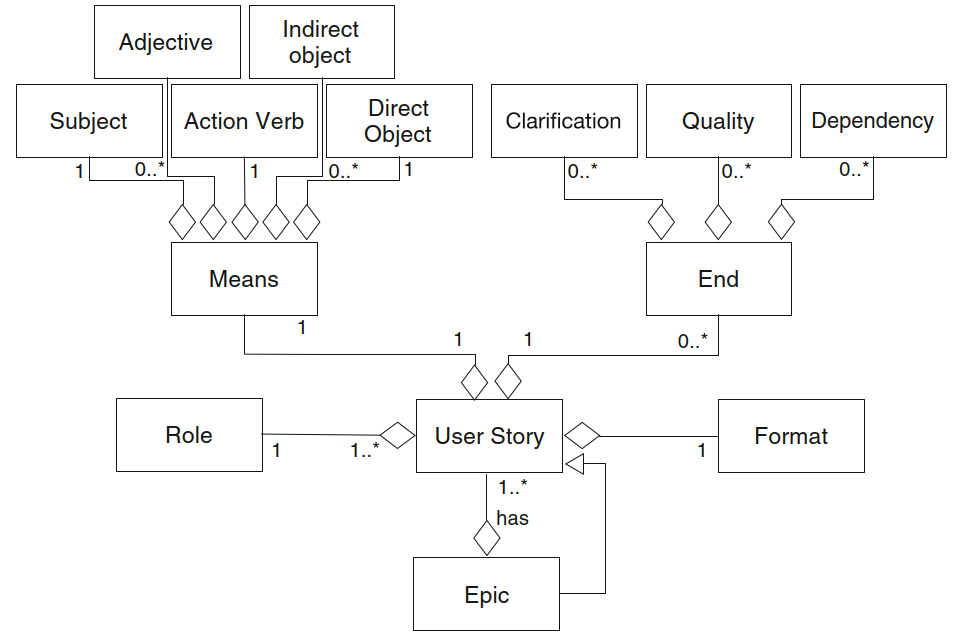
\includegraphics[width=10.03cm, height=7.76cm]{Conceptual_model_of_US}
\caption{Conceptual model of user stories \cite{lucassen2016improving}}\label{fig:conceptual_model}
\end{figure}
\begin{definition}
\emph{Different means, same end }Two or more user stories that have the same end, but achieve this using different means. This relationship potentially impacts two quality criteria, as it may indicate: (1) a feature variation that should be explicitly noted in the user story to maintain an unambiguous set of user stories, or (2) a conflict in how to achieve this end, meaning one of the user stories should be dropped to ensure conflict-free user stories. Formally, for user stories $\mu_1$ and $\mu_2$:\\ 
$diffMeansSameEnd(\mu_1,\mu_2)\leftrightarrow m_1 \neq m_2 \wedge E_1 \cap E_2 \neq \emptyset$
\end{definition}
\begin{definition}
\emph{Same means, different end} Two or more user stories that use the same means to reach different ends. This relationship could affect the qualities of user stories to be unique or independent of each other. If the ends are not conflicting, they could be combined into a single larger user story; otherwise, they are multiple viewpoints that should be resolved. Formally,\\ 
$sameMeansDiffEnd(\mu_1, \mu_2) \leftrightarrow m_1 = m_2 \wedge (E_1 \setminus E_2 \neq \emptyset \vee E_2 \setminus E_1 \neq \emptyset )$
\end{definition}
\begin{definition}
\emph{Full duplicate} $A$ user story $\mu_1$ is an exact duplicate of another user story  $\mu_2$ when the stories are identical. This impacts the unique quality criterion. Formally,\\ 
$isFullDuplicate(\mu_1,\mu_2) \leftrightarrow \mu_1 =_{\text{syn}} \mu_2$
\end{definition}
\begin{definition}
\emph{Semantic duplicate} $A$ user story $\mu_1$ that duplicates the request of $\mu_2$, while using a different text; this has an impact on the unique quality criterion. Formally,\\ 
$isSemDuplicate(\mu_1,\mu_2) \leftrightarrow \mu_1 = \mu_2 \wedge \mu_1 \neq _{\text{syn}} \mu_2$
\end{definition}
\textbf{Uniform}\\ 
Uniformity pertains to the consistency of a USs format, with the majority of user stories within the same set. To evaluate uniformity, the requirements engineer identifies the most frequently occurring format, usually established in collaboration with the team. For example, the US \enquote{As an Administrator, I receive an email notification when a new user is registered} is presented as a non-uniform user story and can be rewritten for improved uniformity as: \enquote{As an Administrator, I want to receive an email notification when a new user is registered.} \\ 
\textbf{Complete}\\ 
The implementation of a set of USs should result in a feature-complete application. While it's not necessary for USs to cover 100\% of the application's functionality up-front, it's crucial not to overlook essential USs, as doing so may create a significant feature gap that hinders progress. For instance, consider the US \enquote{As a User, I am able to edit the content that I added to a person’s profile page}, which requires the existence of another story describing content creation. This scenario can be extended to USs with action verbs that reference non-existent direct objects, such as reading, updating, or deleting an item, which necessitates its creation first. To address these dependencies related to the means' direct object, Lucassen et al. introduce a conceptual relationship. 
\input{Section/USQ_4} 







\section{Extracting Domain Models from Textual Requirements}\label{dmodel}
Automated support for extracting domain models from requirements artefacts such as USs play a central role in effectively supporting the detection of dependencies and conflicts between user stories. Domain models are a simple way to understand the relationship between artefacts and the whole system. 

In this section, we present a comprehensive exploration of techniques that can be employed for the extraction of domain models from agile product backlogs. Furthermore, we conduct a comparative analysis of these techniques. 
\subsection{Visual Narrator: (Automated) Extraction of Conceptual Models form US} \label{vnarrator}
Visual Narrator automatically derive conceptual models from a concise and widely adopted NL notation for USs. Robeer et al. combine NLP heuristics into an algorithm that creates conceptual modes from USs. They present the Visual Narrator as a fully automated, opensource tool that implements the algorithm and generates conceptual models as Web Ontology Languages (OWL) \cite{Robeer2016}.\\ \\ 
\textbf{A Generic Conceptual Model}\\
Robeer et al. define a generic conceptual model of stories that dissects a single US and define its syntactic structure \cite{Lucassen2015}. 

The conceptual model is assembled as a UML class diagram in figure \ref{fig:cmd}. US follow a standard predefined format \cite{Wautelet2014} to capture three distinct aspects of a requirement:
\begin{itemize}
\item Who wants the functionality;
\item What functionality the end users or stakeholders want the system to provide; and 
\item Why the end users and stakeholders need this functionality (optional).
\end{itemize}
These three aspects are captured in a simple textual template to form a running sentence. Although many different templates exist, 70\% of practitioners use the template \enquote{As a \textless type of user\textgreater, I want \textless some goal\textgreater [so that \textless come reason\textgreater ]} \cite{Greer2004}. 
The conceptual model distinguishes between the \emph{role}, \emph{means} and \emph{ends} parts of a US. Each of these parts features an \emph{indicator} which delimits the three basic parts of a US. Jointly, the indicators define the \emph{template} of a user story.

The role part encompasses the role indicator and the \emph{functional} role, describing a generalized type of person \emph{who} interacts with the system. When no ambiguity exists, Robeer et al. use the term \emph{role} to denote both the full part and the \emph{functional role}. The \emph{means} consists of a \emph{subject}, a main \emph{object} of the functionality, and a \emph{main verb} describing the relationship between the subject and main object. The main object can be represented explicitly by the direct object or implicitly (\emph{e.g.}, \enquote{I want to log in} actually, refers to logging in the \emph{system}).

Robeer et al. identified three main purposes that the \emph{ends} may take: (1) clarify the means, (2) reference another user story, or (3) introduce a qualitative requirement.
\begin{figure}
\center
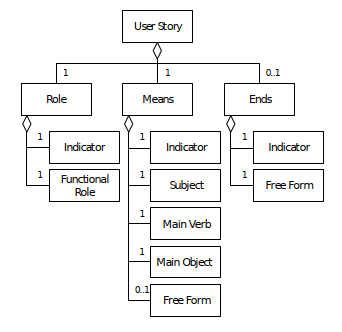
\includegraphics[width=9.03cm, height=7.76cm]{Conceptual_model_defining_the_syntax_of_a_US}
\caption{Conceptual model defining the syntax of a US  \cite{Robeer2016}}\label{fig:cmd}
\end{figure} \\  \\ 
\textbf{The Visual Narrator Tool}\\
To enable the automated extraction of conceptual modes from USs, Robeer et al. developed the \emph{Visual Narrator} tool on the basis of the 11 heuristics \cite{Robeer2016} which takes a set of USs as input and generates a conceptual model as output. The tool only accepts USs that use the indicator as identified by Wautelet \cite{Wautelet2014}: As | \emph{As a(n)} for the role, \emph{I want (to)} | \emph{I can} / \emph{I am able} / \emph{I would like} for the means, and \emph{so that} for the ends part. Syntactically invalid USs are not processed; in order to sanitize these stories, analysts should pre-process them using tools such as AQUSA \cite{lucassen2016improving}.

The architecture of Visual Narrator comprises two main components: (1) the \emph{Processor} and the (2) \emph{Constructor}. The Processor analyzes USs, parsing them into tokens using spaCy \footnote{\href{https://spacy.io/}{\emph{https://spacy.io/}}} and determining token weights based on frequency and user-defined parameters. This results in a \emph{Term-by-User-Story} matrix with weighted terms.

The Constructor then generates a conceptual model from the \emph{WeightedTokens}. It involves the \emph{PatternIdentifier}, which applies heuristics to identify patterns in USs, and the \emph{PatternFactory}, which creates an internal conceptual model based on these patterns and filters out concepts and relationships with weights below a user-specified \emph{threshold}. The Ontology component stores this model, linking parts of it to their originating USs.

To extract a conceptual model from USs, Visual Narrator implements the procedure DERIVECM which takes as input a set of raw user stories \emph{S} and empty sets of concepts \emph{C} and relationships \emph{R}, and populates $C$ and $R$ while parsing the stories and applying the 11 heuristics.

\begin{example}\label{ex_1}
The WebCompany is a young Dutch company that creates tailor-made web business applications. The team consists of nine employees who iteratively develop applications in weekly Scrum sprints. WebCompany supplied 98 user stories covering the development of an entire web application focused on interactive story telling that was created in 2014. 73 of these 98 USs were syntactically correct, usable and relevant for conceptual model generation \cite{lucassen2016improving}. Part of the generated conceptual model is shown in figure \ref{fig:webcompany}.
\begin{figure}
\center
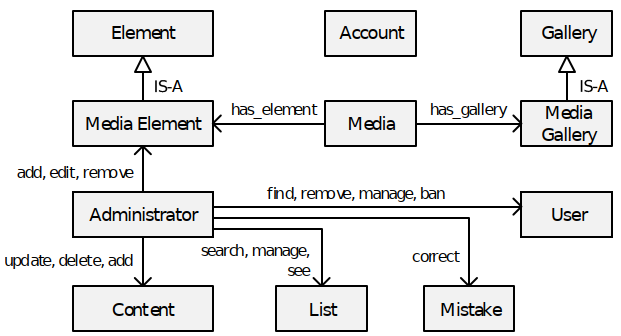
\includegraphics[width=11.03cm, height=5.76cm]{web_company}
\caption{Partial model for WebCompany generated with Visual Narrator   \cite{Robeer2016}}\label{fig:webcompany}
\end{figure}
\end{example} 
\subsection{A Modelling Backlog as Composable Graphs} \label{composable_graph}
Mosser et al. propose a model engineering method (and the associated tooling) to exploit a graph-based meta-modelling and compositional approach. The objective is to shorten the feedback loop between developers and POs while supporting agile development’s iterative and incremental nature. 

The tool can extract what is called a conceptual model of a backlog in an ontology-like way. The conceptual models are then used to measure USs quality by detecting ambiguities or defects in a given story \cite{mosser2022modelling}.
From a modelling point of view, Mosser et al. represents the concepts involved in the definition of a backlog in a metamodel, as depicted in figure \ref{fig:conceptual_metamodel}. Without surprise, the key concept is the notion of story, which brings a Benefit to a \emph{Persona} thanks to an Action performed on an \emph{Entity}. A Story is associated to a readiness \emph{Status}, and might optionally contribute to one or more \emph{QualityProperty} (\emph{e.g.}, security, performance).
\begin{figure}
\center
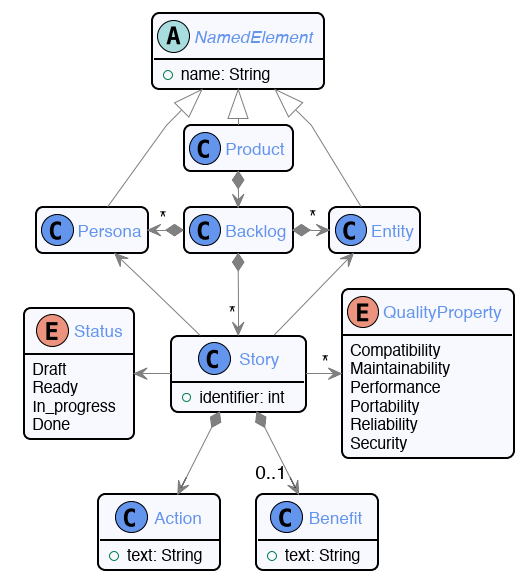
\includegraphics[width=8.03cm, height=8.76cm]{Backlog_conceptual_metamodel}
\caption{Backlog conceptual metamodel \cite{mosser2022modelling}}\label{fig:conceptual_metamodel}
\end{figure}

Consider, for example, the following story, extracted from the reference dataset \cite{Dalpiaz2018}: \enquote{As a user, I want to click on the address so that it takes me to a new tab with Google Maps.}. \emph{This story brings to the user (Persona) the benefit of reaching a new Google Maps tab (Benefit) by clicking (Action) on the displayed address (Entity).}

As Entities and Personas implement the \emph{jargon} to be used while specifying features in the backlog, they are defined at the \emph{Backlog level}. On the contrary, Actions belong to the associated stories and are not shared with other stories. Finally, a \emph{Product} is defined as the \emph{Backlog} used to specify its features.

Mosser et al. propose in the context of backlog management a system which represented in figure \ref{fig:early_feedback} is proposed for utilization. Building upon the efficiency of NLP approaches. Mosser et al. suggest employing an NLP-based extractor to create a backlog model. This model will subsequently assist teams in the planning phase by aiding in the selection of stories for implementation during the upcoming iteration \cite{mosser2022modelling}.
\begin{figure}
\center
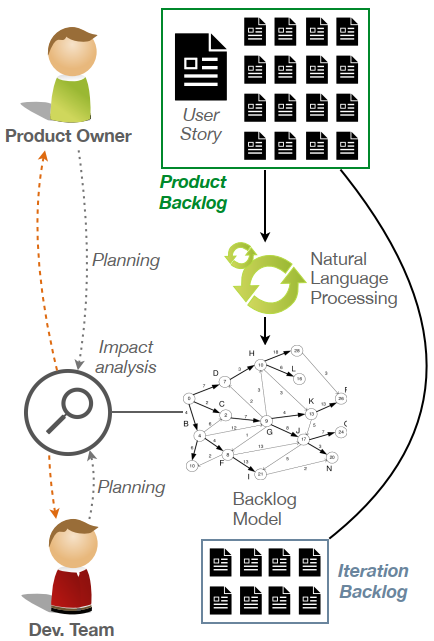
\includegraphics[width=6.03cm, height=8.76cm]{Providing_early_feedback_at_the_backlog_level}
\caption{Providing early feedback at the backlog level \cite{mosser2022modelling}}\label{fig:early_feedback}
\end{figure}\\
\textbf{Composable Backlogs}\\
In order to support team customization (\emph{e.g.}, a given team might want to enrich the backlog metamodel with additional information existing in their product management system) Mossser et al. chose open-world(ontological) representation by modelling backlog as graphs \cite{mosser2022modelling}. The graph is equipped with constraints (\emph{e.g.}, a story always refers to a persona and an entity) to ensure that the minimal structure captured in the previously defined metamodel is guaranteed.
\begin{definition}[\textbf{Story}]
A Story$s \in S$ is defined as a tuple $\left(P,A,E,K\right)$, where $P=\{p_1, ..., p_i\}$ is the set of involved personas, $A= \{a_1, ..., a_i\}$ the set of performed actions, and $E = \{e_1, ..., e_k\}$ the set of targeted entities. Additional knowledge (e.g., benefit, architectural properties, status) can be declared as key-value pairs in $K = \{(k_1,v_1), ..., (k_l,v_l)\}$. The associated semantics is that the declared actions bind personas to entities. Considering that story independence is a pillar of agile methods (as, by definition, stories are independent inside a backlog), there is no equivalence class defined over \\
$S: \forall (s,s')\in S^2, s\neq s' \Rightarrow s \not \equiv s'$.
\end{definition}
\begin{definition}[\textbf{Backlog}]
A backlog $b \in B$ is represented as an attributed typed graph $b = (V, E, A)$, with $V$ a set of typed vertices, $E$ a set of undirected edges linking existing vertices, and $A$ a set of key-value attributes. Vertices are typed according to the model element they represent $v \in V, type(v) \in \{ Persona, Entity, Story \} )$ . Edges are typed according to the kind of model elements they are binding. Like backlogs, vertices and edges can contain attributes, represented as \emph{(key, value)} pairs. The empty backlog is denoted as $\emptyset = (\emptyset ,\emptyset ,\emptyset )$.
\end{definition}
\begin{example}\label{ex_2}
Backlog excerpt: Content Management System for Cornell University — CulRepo \emph{\cite{Dalpiaz2018}}.
\begin{itemize}
\item $s_1$: As a faculty member, I want to access a collection within the repository.
\end{itemize}
Associated model:
\begin{itemize}
\item $s_1 = (\{ faculty member \} ,\{ access\} ,\{ repository, collection\} ,\emptyset)\in S$
\end{itemize}
A backlog containing a single story $s_1$: (\enquote{As a faculty member, I want to access a collection within the repository}). \\ \\ 
$b_1=\left(V_1 , E_1,\emptyset \right ) \in B$ \\ 
$V_1=\left \{ Persona(faculty \ member, \emptyset \right )$ ,

\ \ \ \ $Stroy \left (s_1, \{ \left (action, access \right ) \} \right )$

\ \ \ \ $Entity \left (repository, \emptyset \right ) $,

\ \ \ \ $Entity(collection, \emptyset ) \} $ \\ 
$E_1 = \{ has\_for\_persona(s_1,faculty \ member)$,

\ \ \ \ $has\_for\_entity \left (s_1,repository \right )$

\ \ \ \ $has\_for\_entity(s_1, collection)\}$
\end{example}
\textbf{Conditional Random Fields (CRF)} \\ 
CRFs \cite{Lafferty2001} are a particular class of \emph{Markov Random Fields}, a statistical modelling approach supporting the definition of discriminative models. They are classically used in pattern recognition tasks (labelling or parsing) when context is important identify such patterns \cite{arulmohan2023extracting}.

To apply CRF Mosser et al. transform a given story into a sequence of tuples. Each tuple contains minimally three elements: \emph{(i)} the original word from the story, \emph{(ii)} its syntactical role in the story, and \emph{(iii)} its semantical role in the story. The syntactical role in the sentence is classically known as \emph{Part-of-Speech} (POS), describing the grammatical role of the word in the sentence. The semantical role plays a dual role here. For training the model, the tags will be extracted from the annotated dataset and used as target. When used as a predictor after training, these are the data Mosser et al. will ask the model for infer.

The main limitations of CRF are that \emph{(i)} it works at the word level (model elements can spread across several words), and \emph{(ii)} it is not designed to identify relations between entities \cite{arulmohan2023extracting}.
    To address the first limitation, Mosser et al. use a glueing heuristic. Words that are consecutively associated with the same label are considered as being the same model element, \emph{e.g.}, the subsequence [\enquote{UI}, \enquote{designer}] from the previous example is considered as one single model element of type \emph{Persona}.
    
Mooser et al. applied this heuristic to everything but verbs, as classically, two verbs following each other represent different actions. They used again heuristic approach to address the second limitation. Mooser et al. bound every \emph{Persona} to every primary \emph{Action} (as\emph{ trigger} relations), and every primary \emph{Actions} to every primary \emph{Entity} (as \emph{target} relations) \cite{arulmohan2023extracting}.
\begin{example} Consider the following example:\\ \\
$S=[^\prime As^\prime,^\prime a^\prime,^\prime UI^\prime,^\prime designer^\prime,^\prime,^\prime,\ .\ .\ .]$ \\
$POS(S)=[ADP,DET,NOUN,NOUN,PUNCT,.\ .\ .]$ \\
$Label \left (S \right ) = \left [ \emptyset ,\emptyset ,PERSONA,PERSONA,\emptyset ,.\ .\ .\right ]$ \\\\
$S$ represents a given US (Table \ref{tb:feature_sets}). $POS \left (S \right )$ represent the Part-of-speech analysis of $S$. The story starts with an adposition (ADP), followed by determiner (DET), followed by a noun, followed by another noun, .... Then, $Lables\left (S \right )$ represents what we interest in: the first two words are not interesting, but the $3^{rd}\  and \ 4^{td}$ words represent a Persona.\\ 
\emph{A complete version of the example is provided in Table \ref{tb:feature_sets}.}
\end{example}
\begin{figure}
\center
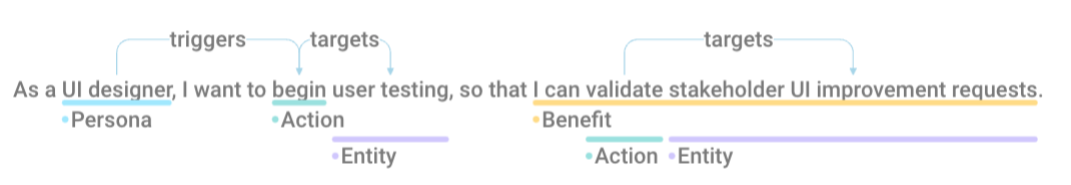
\includegraphics[width=\textwidth, height=2.76cm]{Example_of_annotated_user}
\caption{Example of annotated user using Doccano Annotation UI \cite{arulmohan2023extracting}}\label{fig:annot_usr}
\end{figure}
\begin{figure}
\begingroup
\footnotesize
\begin{tabularx}{\textwidth}{c@{\hspace{4pt}} | c@{\hspace{4pt}}  c@{\hspace{4pt}}  c@{\hspace{4pt}}  c@{\hspace{4pt}}  c@{\hspace{4pt}}  c@{\hspace{4pt}}  c@{\hspace{4pt}}  c@{\hspace{4pt}}  c@{\hspace{4pt}}  c@{\hspace{4pt}}  c@{\hspace{4pt}}  c@{\hspace{4pt}}}
Word &As &a&\textcolor[rgb]{1.0, 0.0, 0.5}{UI}&\textcolor[rgb]{1.0, 0.0, 0.5}{designer}&, &I &want &to&\textcolor[rgb]{0.21, 0.46, 0.53}{begin}&\textcolor[rgb]{0.8, 0.33, 0.0}{user} &\textcolor[rgb]{0.8, 0.33, 0.0}{testing}&,\\
POS&	ADP&	DET	&\textcolor[rgb]{1.0, 0.0, 0.5}{NOUN}	&\textcolor[rgb]{1.0, 0.0, 0.5}{NOUN}	&PUNCT	&PRON	&VERB	&PART	&\textcolor[rgb]{0.21, 0.46, 0.53}{VERB}	&\textcolor[rgb]{0.8, 0.33, 0.0}{NOUN}	&\textcolor[rgb]{0.8, 0.33, 0.0}{NOUN}	&PUNCT \\
Label	&-	&-	&\textcolor[rgb]{1.0, 0.0, 0.5}{PER}	&\textcolor[rgb]{1.0, 0.0, 0.5}{PER}	&-	&-	&-	&-	&\textcolor[rgb]{0.21, 0.46, 0.53}{P-ACT}	&\textcolor[rgb]{0.8, 0.33, 0.0}{P-ENT}	&\textcolor[rgb]{0.8, 0.33, 0.0}{P-ENT}	&- \\
 \end{tabularx}
  \begin{tabularx}{\textwidth}{c}
  \\
  \end{tabularx}
 \begin{tabularx}{\textwidth}{c@{\hspace{4pt}} | c@{\hspace{4pt}}  c@{\hspace{4pt}}  c@{\hspace{4pt}}  c@{\hspace{4pt}}  c@{\hspace{4pt}}  c@{\hspace{4pt}}  c@{\hspace{4pt}}  c@{\hspace{4pt}}  c@{\hspace{4pt}}  c@{\hspace{4pt}}  c@{\hspace{4pt}}  c@{\hspace{4pt}}}
Word&	so	&that	&I	&can	&\textcolor[rgb]{0.09, 0.45, 0.27}{validate}	&\textcolor[rgb]{0.5, 0.0, 0.5}{stakeholder}	&\textcolor[rgb]{0.5, 0.0, 0.5}{UI}	&\textcolor[rgb]{0.5, 0.0, 0.5}{improvement}	&\textcolor[rgb]{0.5, 0.0, 0.5}{requests}	&. \\
POS	&SCONJ	&SCONJ	&PRON	&AUX	&\textcolor[rgb]{0.09, 0.45, 0.27}{VERB}	&\textcolor[rgb]{0.5, 0.0, 0.5}{NOUN}	&\textcolor[rgb]{0.5, 0.0, 0.5}{NOUN}	&\textcolor[rgb]{0.5, 0.0, 0.5}{NOUN}	&\textcolor[rgb]{0.5, 0.0, 0.5}{NOUN}	&PUNCT\\
Label	&-	&-	&-	&-	&\textcolor[rgb]{0.09, 0.45, 0.27}{S-ACT}	&\textcolor[rgb]{0.5, 0.0, 0.5}{S-ENT}	&\textcolor[rgb]{0.5, 0.0, 0.5}{S-ENT}	&\textcolor[rgb]{0.5, 0.0, 0.5}{S-ENT}	&\textcolor[rgb]{0.5, 0.0, 0.5}{S-ENT}	&-\\
 \end{tabularx} \\ \\ 
\scriptsize \emph{POS tags are the Universal POS tags \\ 
Labels: PER (Persona), P-ACT (Primary Action), P-ENT (Primary Entity), S-ACT (Secondary Action), S-ENT (Secondary Entity)}
\begin{TableCaption}
\caption{Minimal Feature Set, associating part-of-speech (POS) and semantic labels to each word in a given story \cite{arulmohan2023extracting}}\label{tb:feature_sets}
\end{TableCaption}
\endgroup
\end{figure}
\subsection{Extracting Domain Models with GPT 3.5} \label{sec_gpt}
Mooser et al. experimented with ChatGPT to find the best way to extract the information from a US backlog in a \emph{\enquote{rapid prototyping}} way. They initially used a batch approach to extract information from stories using a GPT agent. However, they faced limitations due to token limits and hallucinations. To address this, they switched to a one-by-one story approach, reducing hallucinations but still producing unusable results. 

They then explored function calls introduced in \emph{gpt-3.5-turbo-0613} \footnote{\href{https://platform.openai.com/docs/guides/gpt/completions-api}{https://platform.openai.com/docs/guides/gpt/completions-api}}, allowing control over output which make developer able to provide a JSON schema in order to model their response, and the system will use this schema and \emph{\enquote{fill in the blanks}} instead of regular text generation.
\begin{example}
If one expects their answer to be an array of strings containing the name of the personas, they can provide a schema inside their request, and GPT will use it as output format (as in Figure \ref{fig:calling_gpt}, line $3 \rightarrow  12$). An example of such a constrained response is described in Figure \ref{fig:gpt_answer}.
\begin{figure}
\begin{lstlisting}[language=json,firstnumber=1]
response = openai.ChatCompletion.create(
    model = "gpt-3.5-turbo-0613",
    functions = [ #constraining_GPT_with_a_schema
	{ "name": "record_elements", #Function to be called in the response
	  "description": "Record_the_elements_extracted_from_a_story",
	  "parameters": { #Signature_description
		"type": "object",
		"properties": {
		"personas": {
			"type": "array",
			"description": "The list of personas extracted from the story",
			"items": { "type": "string" }}}],
    messages = conv,
    temperature=0.0) #To_make_the_answer_deterministic_(as_much_as_possible)
\end{lstlisting}
\caption{Calling GPT 3.5 and specifying a function call argument  \cite{arulmohan2023extracting}}\label{fig:calling_gpt}
\end{figure}
\begin{figure}
\begin{lstlisting}[language=json,firstnumber=1]
{
    ...
    "choices": [{
    	"index": 0, "message": {
	 "role": "assistant", "content": null,
	 "function_call": {
	    "name": "record_elements",
          	    "arguments":
	         "{\"personas\": [\"repository manager\"]}"
    }},
 "finish_reason": "function_call"}],
    ...
}
\end{lstlisting}
\caption{Example of answer from the API (execution of Figure \ref{fig:calling_gpt})  \cite{arulmohan2023extracting}}\label{fig:gpt_answer}
\end{figure}
\end{example}
To address limitations in GPT's output format control, the Mosser et al. introduced the option to use JSON schemas in requests, allowing users to specify the desired output format. They also explored the use of function calls as responses but found it impractical due to conversation termination. Faced with this, they had two options: defining a large schema or engaging in a conversation with the model. They chose the latter, designing the processing of each story as a conversation with a smaller, dedicated schema.
Eventually, they adopted a conversation-based approach with smaller JSON schemas to process each story effectively. 
They organized the conversation into four phases:
\begin{enumerate}
\item Setup. First, the system role will be impersonated and ask the engine to adopt a persona. 
\item Concepts. The task of extracting personas, entities, actions and benefit from a story will be proceed.
\item Categorization. Given stateless of the model, it becomes necessary to inject the answer obtained from the preceding phase into the ongoing conversation. Consequently, Mooser et al. assume the role of the assistant and include a conversation entry detailing the  \textless CONCEPTS\textgreater \ obtained in the previous phase. Following the established pattern from the prior phase, Mooser et al. articulate the task using the system role, which entails categorizing primary and secondary actions and entities.
\item Relations. The final step uses the same pattern. Mosser et al. first inject the \textless CATEGORIES\textgreater \ as the assistant, and then describe the task and provide an example as the system.
\end{enumerate}


\subsection{Comparative Analysis} \label{comparative_analysis}
In this subsection we consider a comparative analysis of mentioned methodologies to discern the most suitable approach for our specific context.

In the context of evaluating three approaches (Visual Narrator, GPT-3.5, and Conditional Random Fields or CRF) for the task of domain concept extraction from a corpus of stories, it is evident that CRF emerges as a compelling choice. Here are the reasons why CRF should be chosen for our approach:
\begin{itemize}
\item Tailored Approach: Mosser et al. highlights CRF as a rule-based approach, allows for a tailored and domain-specific model. This tailored approach is crucial when dealing with complex domain-specific tasks like concept extraction. CRF can be fine-tuned by domain experts to address the specific challenges of the task.
\item Training Requirement: CRF requires training, it was trained using a classical 80/20 separation method. This training phase allows CRF to learn the patterns and relationships between domain concepts and the textual context. This training can lead to improved accuracy and relevance in domain concept extraction (Figure \ref{fig:coparing_approaches}) \cite{arulmohan2023extracting}.
\item Model Complexity: In comparison to other approaches, CRF's implementation is relatively simple, and it requires a smaller codebase. This simplicity makes it easier to manage and maintain, reducing the complexity associated with more extensive models like GPT-3.5.
\item $F-measure\ (F_1)$ : Mosser et al. measures performance using the $F_1$ score, which is particularly suitable for this task. $F_1$ considers both precision and recall, which is essential when dealing with domain concept extraction. It is well-suited for situations where false positives and false negatives have different costs \cite{arulmohan2023extracting}.
\item Superior Performance: Empirical results indicate that CRF consistently outperformed other approaches, including GPT-3.5, in all evaluation criteria. CRF achieved the highest $F_1$ scores, particularly for Persona's extraction, reaching a perfect score of 1.0 which means a perfect match (score of 0.0 means that precision or recall is null). This superior performance is indicative of CRF's effectiveness in this specific task \cite{arulmohan2023extracting}.
\item Reproducibility: CRF offers transparency and interpretability, making it easier to understand and reproduce results compared to more opaque machine learning models.
\item Concerning the Agile DevOps Paradigms: Visual Narrator keeps its conceptual model internal and exposes black-box analysis to users, dedicated to stories quality in terms of requirements engineering, for example. Thus, it does not support the DevOps team in the development, as the provided feedback focuses on the requirements expression instead of their role in the software development. CRF instead leverage the graph structure of the ontologies and exploit a graph-based meta-modelling and compositional approach to shorten the feedback loop between developers and Ops while supporting agile development’s iterative and incremental nature \cite{mosser2022modelling}.
\item Syntactic and semantic Covering: In contrast to GPT-3.5 and CRF, which consider both the syntactic and semantic aspects of US, NLP has constrained its focus solely to the syntactic structure of the US.
\end{itemize}
\begin{figure}
\center
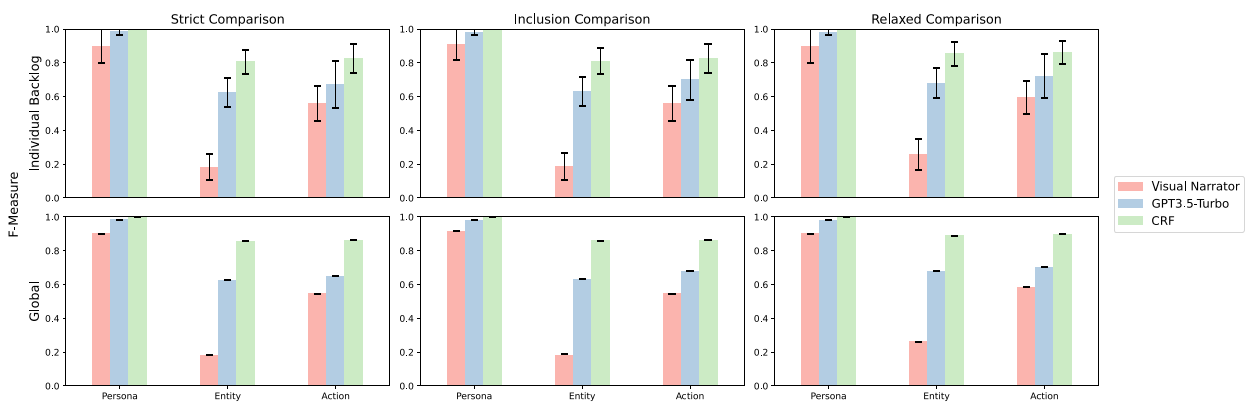
\includegraphics[width=\textwidth, height=5.76cm]{Comparing_approaches_to_the_ground_truth}
\caption{Comparing approaches to the ground truth: $F-measure \ (F_1)$ results for Visual Narrator, CRF and GPT-3.5  \cite{arulmohan2023extracting}}\label{fig:coparing_approaches}
\end{figure}
\subsection{Bottom Line}\label{crf_bottom_line}
We have chosen the Conditional Random Fields (CRF) approach because of their graph-based nature and their significant promise in terms of precision and recall, which is particularly important in the context of domain concept extraction. CRF can cover both syntactic and semantic aspects, especially when complemented by an appropriate conceptual metamodel, which makes it suitable for definition as a type graph in Henshin. The annotations generated by CRF can then be used for transformation into a rule-based graph transformation system, improving support for DevOps practices.






\section{NLP and Computational Lexical Resource Techniques}\label{nlp}
Natural language processing (NLP) is a computational method for the automated analysis and representation of human language \cite{cambria2014jumping}. NLP techniques offer potential advantages to improve the quality of USs and can be used to parse, extract, or analyze user story's data. It has been widely used to help in the software engineering domain (\emph{e.g.}, managing software requirements \cite{Arias2018}, extraction of actors and actions in requirement document \cite{al2018use}.

NLP techniques are usually used for text preprocessing (\emph{e.g.}, tokenization, \emph{Part-of-Speech} (POS) tagging, and dependency parsing). Several NLP approaches can be used (\emph{e.g.}, syntactic representation of text and computational models based on semantic features). Syntactic methods focus on word-level approaches, while the semantic focus on multiword expressions \cite{cambria2014jumping}.

A computational lexicon resource is a systematically organized repository of words or terms, complete with linguistic and semantic data. These lexicons play a pivotal role in facilitating NLP systems focused on semantic analysis by offering comprehensive insights into language elements, encompassing word forms, part-of-speech (POS) categories, phonetic details, syntactic properties, semantic attributes, and frequency statistics. Lexical classes, defined in terms of shared meaning components and similar (morpho-) syntactic behavior of words, have attracted considerable interest in NLP \cite{cambria2014jumping}. These classes are useful for their ability to capture generalizations about a range of (cross-) linguistic properties. NLP systems can benefit from lexical classes in a number of ways. As the classes can capture higher level abstractions (\emph{e.g.} syntactic or semantic features) they can be used as a principled means to abstract away from individual words when required. Their predictive power can help compensate for lack of sufficient data fully exemplifying the behavior of relevant words \cite{kipper2006extending}.

Upon the completion of the transformation of USs utilizing a Conditional Random Fields (CRF) approach, wherein entities, actions (both primary and secondary), persona, and their relational attributes (specifically, triggers, targets and contains) are meticulously annotated and structured as a graph-based representation, a preliminary imperative emerges. This imperative entails the determination of a representative semantic interpretation for the ascertained actions. This determination, in turn, serves as a prerequisite for the generation of corresponding transformation rules, namely, \enquote{create}, \enquote{delete} and \enquote{forbidden} rules.

The attainment of this representative semantic interpretation hinges upon the application of a suite of foundational lexical resource techniques of a conceptual nature. These techniques assume a pivotal role in furnishing the essential cognitive infrastructure, facilitating a comprehensive grasp of the semantic roles, syntactic characteristics, and the systematic categorization to \enquote{creation}, \enquote{deletion} and \enquote{forbiddance} of linguistic elements embedded within the construct of the US.

Next, we will undertake a systematic examination of various computational lexical resource techniques. Subsequently, we will conduct a comparative analysis to determine the optimal approach for integration into our approach. 
\subsection{WordNet} \label{wordnet}
WordNet is an online lexical database designed for use under program control. English nouns, verbs,
adjectives, and adverbs are organized into sets of synonyms, each representing a lexicalized concept. Semantic relations link the synonym sets \cite{miller1990introduction}. 

WordNet operates by classifying words into four core syntactic categories: nouns, verbs, adjectives, and adverbs, collectively referred to as open-class words (see Table \ref{tb:wordnet}). This categorization allows for versatile language analysis and interpretation. For instance, words like "back," "right," or "well" can be interpreted differently based on their linguistic context, and thus, WordNet separately incorporates these varied interpretations \cite{miller1995wordnet}.

WordNet not only addresses word forms but also considers their inflectional morphology, accommodating the linguistic nuances that can arise due to different syntactic categories. For instance, when information is sought for \enquote{went}, the system intelligently provides relevant details about the verb \enquote{go}. On the other hand, derivational and compound morphology, encompassing words like \enquote{interpret}, \enquote{interpreter}, \enquote{misinterpret}, and so forth, are acknowledged as distinct entities within WordNet, despite sharing a common root.

One of WordNet's key strengths lies in its incorporation of various semantic relations, meticulously chosen to serve the broader scope of the English language. These relations are designed to be user-friendly and intuitively understandable, making them accessible even to individuals without advanced linguistic training. WordNet's semantic relations encompass \cite{miller1995wordnet}:
\begin{itemize}
\item Synonymy: The fundamental relation in WordNet, which employs sets of synonyms (synsets) to encapsulate word senses. This relation is symmetric and connects different word forms that share the same sense.
\item Antonymy (opposing-name): A symmetric relation that highlights opposing word forms, particularly vital in organizing the meanings of adjectives and adverbs.
\item Hyponymy (sub-name) and Hypernymy (super-name): These transitive relations between synsets organize noun meanings into hierarchical structures, with hypernyms representing broader categories and hyponyms representing specific instances or subcategories.
\item Meronymy (part-name) and Holonymy (whole-name): These complex relations delineate the component parts, substantive parts, and member parts of various concepts within WordNet.
\item Troponymy (manner-name): Similar to hyponymy but applicable to verbs, troponymy results in hierarchies that are typically shallower.
\item Entailment Relations: WordNet also accounts for entailment relations between verbs, capturing the logical inferences that can be drawn from certain actions.
\end{itemize}
These semantic relations are represented in WordNet through pointers, establishing connections between word forms and synsets. In total, WordNet incorporates more than 116,000 of these pointers, facilitating the exploration of intricate semantic relationships.
\begin{figure}
\begingroup
\footnotesize
\centering
\begin{tabularx}{10cm}{l  c  l}
\hline
Semantic Relation	& Syntactic Category	& Example \\
\hline
\hline
Synonymy (similar) &	N, V, Aj, Av	&  pipe , tube \\
 & & rise, ascend \\
  & & sad, unhappy \\
  & & rapidly, speedily \\\\ 
\hline
Antonymy (opposite)&	Aj, Av, (N, V)	&wet, dry \\
& & powerful, powerless \\
 & & friendly, unfriendly\\
 & & rapidly, slowly \\\\ 
 \hline
Hyponymy (subordinate)	&N	&sugar maple, maple \\
&&maple, tree\\
&&tree, plant\\\\ 
\hline
Meronymy (part)	&N	&brim, hat \\
&&gin, martini\\
&&ship, fleet\\\\ 
\hline
Troponomy(manner)&	V	&march, walk\\
&&whisper, speak\\
\hline
Entailment	&V	&drive, ride\\
&&divorce, marry\\\\ 
\hline
\\ 
\multicolumn{3}{c}{Note:     N = Nouns     Aj = Adjectives     V = Verbs     Av = Adverbs} \\
\hline
\end{tabularx}
\begin{TableCaption}
\caption{Semantic Relation in WordNet  \cite{miller1995wordnet}}\label{tb:wordnet}
\end{TableCaption}
\endgroup
\end{figure}

\subsection{FrameNet} \label{framenet}
The Berkeley FrameNet project is dedicated to creating machine-readable semantic descriptions for a multitude of English words. The project's primary goal is to encode human semantic knowledge into machine-readable formats, guided by empirical findings from corpus-based research. The project ambitiously covers various semantic domains, such as HEALTH CARE, CHANCE, PERCEPTION, COMMUNICATION, TRANSACTION, TIME, SPACE, BODY, MOTION, LIFE STAGES, SOCIAL CONTEXT, EMOTION, and COGNITION. The Berkeley FrameNet project plays a significant role in advancing natural language understanding and semantic analysis \cite{baker1998berkeley}.

The Berkeley FrameNet project yields two crucial outcomes: the FrameNet database and associated software tools. The database comprises three major components:
\begin{itemize}
\item Lexicon: This section includes entries containing conventional dictionary-type data for human readers' comprehension. It also incorporates FORMULAS, which capture the morphosyntactic structures within phrases or sentences built around words. Links to semantically ANNOTATED EXAMPLE SENTENCES illustrate these realization patterns found in the formulas. Additionally, there are connections to the FRAME DATABASE and other machine-readable resources like WordNet and COMLEX.
\item Frame Database: This component provides descriptions of each frame's basic conceptual structure, offering names and descriptions for the elements participating in these structures. Table \ref{tb:framenet} schematizes several related entries in this database \cite{baker1998berkeley}.
\item Annotated Example Sentences: These sentences are marked up to showcase both semantic and morphosyntactic properties of lexical items. These sentences lend empirical support to the lexicographic analyses found in the frame database and lexicon entries.
\end{itemize}
These three components are tightly integrated, with elements in each able to reference elements in the other two. Moreover, the database will include estimates of the relative frequency of senses and complementation patterns by comparing the senses and patterns in hand-tagged examples with the entire BNC corpus \cite{baker1998berkeley}.
\begin{figure}
\begingroup
\footnotesize
\centering
\begin{tabularx}{8cm}{l}
\hline
frame (TRANSPORTATION) \\
frame.elements (MOVER(S), MEANS, PATH)\\
scene (MOVER(S) move along PATH by MEANS)\\
\hline
frame (DRIVING)\\
inherit (TRANSPORTATION)\\
frame.elements (DRIVER (=MOVER), VEHICLE)\\
(=MEANS), RIDER(S) (=MOVER(S)), CARGO)\\
(=MOVER(s)))\\
scenes (DRIVER starts VEHICLE, DRIVER controls\\
VEHICLE, DRIVER stops VEHICLE)\\
\hline
frame ($RIDING_1$)\\
inherit (TRANSPORTATION)\\
frame\_elements (RIDER(S) (=MOVER(S)), VEHICLE\\
 (=MEANS))\\
scenes (RIDER enters VEHICLE, VEHICLE carries\\
 RIDER along PATH, RIDER leaves VEHICLE)\\
\hline
\end{tabularx}
\begin{TableCaption}
\caption{A subframe can inherit elements and semantic from its parent  \cite{baker1998berkeley}}\label{tb:framenet}
\end{TableCaption}
\endgroup
\end{figure}
\subsection{VerbNet} \label{verbnet}
VerbNet (VN) is a hierarchical domain-independent, broad-coverage verb lexicon with mappings to several widely-used verb resources, including WordNet \cite{miller1995wordnet}, Xtag \cite{prolo2002generating}, and FrameNet \cite{baker1998berkeley}. It includes syntactic and semantic information for classes of English verbs derived from Levin’s classification which is considerably more detailed than that included in the original classification. 

Each verb class in VN is completely described by a set of members, thematic roles for the predicate-argument structure of these members, selectional restrictions on the arguments, and frames consisting of a syntactic description and semantic predicates with a temporal function, in a manner similar to the event decomposition of Moens and Steedman \cite{moens2005temporal}. The original Levin classes have been refined and new subclasses added to achieve syntactic and semantic coherence among members. \\
\textbf{Syntactic Frames} \\ 
Semantic restrictions, such as constraints related to animacy, humanity, or organizational affiliation, are employed to limit the types of thematic roles allowed within these classes. Furthermore, each syntactic frame may have constraints regarding which prepositions can be used. 

Additionally, there may be additional constraints placed on thematic roles to indicate the likely syntactic nature of the constituent associated with that role.
Levin classes are primarily characterized by NP (noun phrase) and PP (prepositional phrase) complements. 

Some classes also involve sentential complementation, albeit limited to distinguishing between finite and non-finite clauses. This distinction is exemplified in VN, particularly in the frames for the class Tell-37.2, as shown in Examples (1) and (2), to illustrate how the differentiation between finite and non-finite complement clauses is implemented.
\begin{enumerate}
\item Sentential Complement (finite): \\ \ \ \enquote{Susan told Helen that the room was too hot.} \\ \emph{Agent V Recipient Topic [+sentential – infinitival]}
\item Sentential Complement (nonfinite): \\ \ \  \enquote{Susan told Helen to avoid the crowd.}\\ \emph{Agent V Recipient Topic [+infinitival – wh\_inf]}
\end{enumerate}
\textbf{Semantic Predicates}\\ 
Each VN frame also contains explicit semantic information, expressed as a conjunction of Boolean semantic predicates such as \enquote{motion}, \enquote{contact}, or \enquote{cause}. Each of these predicates is associated with an event variable E that allows predicates to specify when in the event the predicates are true $start(E)$ for preparatory stage, $during(E)$ for the culmination stage, and $end(e)$ for the consequent stage). 

Relations between verbs (or classes) such as antonymy and entailment present in WordNet and relations between verbs (and verb classes) such as the ones found in FrameNet can be predicted by semantic predicates. Aspect in VN is captured by the event variable argument present in the predicates.\\ 
\textbf{The VerbNet Hierarchy}\\ 
VerbNet represents a hierarchical structure of verb behavior, with groups of verb classes sharing similar semantics and syntax. Verb classes are numbered based on common semantics and syntax, and classes with the same top-level number (e.g., 9-109) have corresponding semantic relationships. 

For instance, classes related to actions like \enquote{putting}, such as \enquote{put-9.1}, \enquote{put\_spatial-9.2}, \enquote{funnel-9.3}, all belong to class number 9 and relate to moving an entity to a location. Classes sharing a top class can be further divided into subclasses, as seen with \enquote{wipe} verbs categorized into \enquote{wipe\_manner} $(10.4.1)$ and \enquote{wipe\_inst} $(10.4.2)$ specifying the manner and instrument of \enquote{wipe} verbs in the \enquote{Verbs of Removing} group of classes (class number 10).

The classification encompasses class numbers 1-57, derived from Levin's classification \cite{levin1993english}, and class numbers 58-109, developed later by Korhonen and Briscoe \cite{korhonen2004extended}. The later classes are more specific, often having a one-to-one relationship between verb type and verb class. This hierarchical structure helps categorize and organize verbs based on their semantic and syntactic properties.\\ 
\textbf{Verb Class Hierarchy Contents}\\ 
Each individual verb class within VerbNet is hierarchical. These classes can include one or more \enquote{subclasses} or \enquote{child} classes, as well as \enquote{sister} classes. All verb classes have a top-level classification, but some provide further specification of the behaviors of their verb members by having one or more subclasses. 

Subclasses are identified by a dash followed by a number after the class information. For example, the top class might be \enquote{spray-9.7}, and a subclass would be denoted as \enquote{spray 9.7-1}. This hierarchy allows for a more detailed and structured organization of verb behavior within VerbNet. 
\begin{itemize}
\item \textbf{Top Class:} The highest class in the hierarchy; all features in the top class are shared by every verb in the class. The top class of the hierarchy consists of syntactic constructions and semantic role labels that are shared by all verbs in this class.
\item \textbf{Parent Class:} Dominates a subclass; all features are shared with subordinate classes.
\item \textbf{Subclasses:} VerbNet subclasses inherit features from the top class but specify further syntactic and semantic commonalities amongst their verb members. These can include additional syntactic constructions, further selectional restrictions on semantic role labels, or new semantic role labels.
\item \textbf{Child Class:} Is dominated by a parent class; inherits features from this parent class, but also adds information in the form of additional syntactic frames, thematic roles, or restrictions. 
\item \textbf{Sister Class:} A subclass directly dominated by a parent class. This parent class also, directly dominates another subclass, so the two subclasses are sisters to one another. Sister classes do not share features.
\end{itemize}
Figure \ref{fig:hierachy_class} illustrate an example of class hierarchy form spray-9.7 class.
\begin{figure}
\center
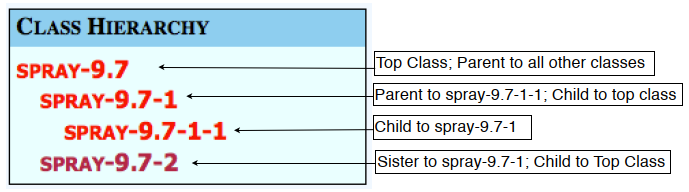
\includegraphics[width=11.03cm, height=2.76cm]{Class_hierarchy_for_spray-9_punk_7_class}
\caption{Class hierarchy for spray-9.7 class \cite{heck2014quality}}\label{fig:hierachy_class}
\end{figure}
Verb Classes are numbered according to shared semantics and syntax, and classes which share a top-level number (9-109) have corresponding semantic relationships. 

For instance, verb classes related to putting, such as put-9.1, put\_spatial-9.2, funnel-9.3, etc. are all assigned to the class number 9 and related to moving an entity to a location. 

Classes that share a top class can also be divided into subclasses, such as wipe verbs in wipe\_manner (10.4.1) and wipe\_inst (10.4.2) which specify the manner and instrument of wipe verbs in the \enquote{Verbs of Removing} group of classes (class number 10). 

An example of top-class numbers and their corresponding types is given in Table \ref{tb:vtype_example}. Class numbers 1-57 are drawn directly from Levin's (1993) classification. Class numbers 58-109 were developed later in the work of Korhonen \& Briscoe (2004). Notably, the verb types of the later classes are less general, as indicated by the fact that most of these classes have a one-to-one relationship between verb type and verb class.

\begin{figure}
\begingroup
\footnotesize
\centering
\begin{tabularx}{12cm}{l  l  l}
\hline
Class Number	&Verb Type	&Verb Class \\
\hline 
\hline
10&	Verbs of Removing		&banish-10.2 \\
&&cheat-10.6.1\\
&&clear-10.3\\
&&debone-10.8\\
&&fire-10.10\\
&&mine-10.9\\
&&pit-10.7\\
&&remove-10.1\\
&&resign-10.11\\
&&steal-10.5\\
&&wipe\_manner-10.4.1\\
\hline
26	&Verbs of Creation and Transformation	&adjust-26.9 \\
&&build-26.1 \\
&&convert-26.6.2\\
&&create-26.4\\
&&grow-26.2.1\\
&&knead-26.5\\
&&performance-26.7\\
&&rehearse-26.8\\
&&turn-26.6.1\\
\hline
13&	Verbs of Change of Possession	&berry-13.7 \\
&&contribute-13.2\\
&&equip-13.4.2\\
&&exchange-13.6.1\\
&&fulfilling-13.4.1\\
&&future\_having-13.3\\
&&get-13.5.1\\
&&give-13.1\\
&&hire-13.5.3\\
&&obtain-13.5.2\\
\hline
\end{tabularx}
\begin{TableCaption}
\caption{An example of top-class numbers and their corresponding verb-type\cite{verbnet_guidelines}}\label{tb:vtype_example}
\end{TableCaption}
\endgroup
\end{figure}
\subsection{Comparative Analysis} \label{sec_5_campare}
After a careful comparative analysis of WordNet, FrameNet, and VerbNet, we have determined that VerbNet is the most suitable lexical resource for our project. Its hierarchical categorization of verbs into classes provides a structured and comprehensive approach to understanding verb behavior, which is essential for our goal of generating transformation rules based on semantic interpretations of actions within user stories. 

VerbNet's organization aligns seamlessly with our project's requirements, offering the precision and granularity required for our semantic analysis and rule generation tasks.
Here are the three comparison key aspects:
\begin{itemize}
\item Focus: VerbNet is specialized in verbs, FrameNet offers broader coverage, including nouns and adjectives, and WordNet covers a wide range of words across different parts of speech.
\item Hierarchy: VerbNet and FrameNet provide hierarchical structures that help organize and understand word behavior, while WordNet focuses on synsets and relationships between words.
\item Applications: VerbNet is ideal for tasks related to verb semantics and actions. FrameNet is versatile for various lexical semantic tasks, and WordNet is widely used for word sense disambiguation and related applications.
\end{itemize}
\subsection{Conclusion}\label{nlp_bottom_line}
For our approach we identified VerbNet as the most appropriate lexical resource. Its methodical categorisation of verbs into hierarchical classes provides a structured and all-encompassing framework for understanding verb behavior. This alignment with our project goals is of utmost importance as it underpins our task of formulating transformation rules based on semantic interpretations of the actions (verbs) recognised by CRF and described in USs. VerbNet's organizational structure seamlessly matches the requirements of our project and ensures the necessary precision and granularity that are essential for our semantic analysis and rule generation.


\section{Analysis by Graph Transformation Tools}\label{gts}
In this section, some basic definitions about graph transformation and transformation rules are first established for better understanding. Afterwards, we dive into graph transformation tools, which play a pivotal role in our methodology. 

In a software development process, the class architecture is getting changed over the development, \emph{e.g.} due to a change of requirements, which results in a change of the class diagram. During runtime of a software an object diagram can also be modified trough creating or deleting of new objects. 

Many structures, that can be represented as graph are able change or mutate. This suggests the introduction of a method to modify graphs through the creation or deletion of nodes and edges. This graph modification can be performed by the so-called graph transformations. There are many approaches to model graph transformations \emph{e.g.} the double pushout approach or the single pushout approach which are both concepts based on pushouts from category theory in the category Graphs.\\ 
\textbf{Graphs and Typed Graphs}\\ 
A graph is comprised of nodes and edges, with each edge connecting precisely two nodes and having the option to be directed or undirected. When an edge is directed, it designates a distinct start node (source) and an end node (target). For the purpose of this discussion, we will focus on directed graphs.

\begin{definition}[\textbf{graph}]
\label{def_graph}
A \emph{graph} $G = (V,E,s,t)$ contains $V$, a set of nodes, $E$, a set of edges, $s: E \to V$, a source function, where $s(e)$ is the start node of $e \in E$ and a target function $t:E \to V$, where $t(e)$ is the end node of a edge $e \in E$.
\end{definition}

\begin{definition}[\textbf{Transformation Rule}]
A \emph{transformation rule} denotes which nodes and edges of a graph have to be deleted and which nodes and edges have to be created.
In the double-pushout approach a transformation rule $p = L \xhookleftarrow{l} K \xhookrightarrow{r} R$ consists of three graphs $L,K,R$, two graph morphisms $l: K \to L$ and $r: K \to R$, where $K$ contains all elements, that remain in the graph, $L \setminus l(K)$ contains the elements that are removed and $R \setminus r(K)$ contains the elements, that are created.
\end{definition}
\begin{definition}[\textbf{Graph Transformation}]
In the context of \emph{graph transformations}, when we have two graphs $G$ and $H$, along with a transformation rule $p$, we can apply this rule to graph $G$ at match $m$. This application, denoted as $G \xRightarrow{p,m} H$, results in graph $H$. The match, represented as $m : L \hookrightarrow G$, is an injective graph morphism, and $L$ contains all the nodes and edges of $p$ that remain intact and are not deleted during the transformation.
\end{definition}
As outlined in Section \ref{dmodel}, where we elucidated our utilization of Conditional Random Fields (CRF) as a graph-based metamodeling and compositional approach for annotating USs, each US is meticulously structured and annotated in the form of a graph. Subsequently, we will apply transformation rules to these CRF-generated graphs to modelling graph transformation.

To accomplish this objective, we have harnessed the capabilities of established lexical resources such as VerbNet. This utilization of VerbNet enables us to categorize actions (which are verbs) extracted from the US into three distinct categories, namely: \enquote{create}, \enquote{delete}, \enquote{forbid}. These categories serve as essential components of transformation rules that articulate precise changes within the graph-based representation. 

In the following subsections, we will introduce two prominent graph transformation tools, Groove and Henshin, shedding light on their respective capabilities and applicability within our CRF-driven metamodeling framework for US annotation and transformation. Finally, we illustrate comparative analysis of the most suitable tool for our specific use case.
\subsection{GROOVE: Modelling and analysis Tool}\label{groove}
Graphs in groove consist of labelled nodes and edges. An edge is a binary arrow between two nodes. Node labels can either be node types or flags; the latter can be used to model a Boolean condition, which is true for a node if the flag is there and false if it is absent.

GROOVE can work either in an untyped or in a typed mode. In the untyped mode, graphs can be arbitrary: there are no constraints on the allowed combinations of node types, flags and edges. In the typed mode, all graphs and rules must be well-typed, meaning that they can be mapped into a special type graph. This is checked statically for the start graph and the rules: the theory then ensures that well-typedness is preserved under transformation. The type graph determines the allowed combinations of node types and edges \cite{ghamarian2012modelling}.\\ 
\textbf{Rules and Application Condition}\\ 
Graphs are transformed by applying rules. A rule consists of the following:
\begin{itemize}
\item A pattern that must be present in the host graph in order for the rule to be applicable
\item Subpatterns that must be absent in the host graph in order for the rule to be applicable
\item Elements (nodes and edges) to be deleted from the graph
\item Elements (nodes and edges) to be added to the graph
\item Pairs of nodes that are to be merged
\end{itemize}
All these elements are combined into a single graph; colors and shapes are used to distinguish them. Ghamarian et al. distinguish positive (which must be present in order to apply a rule) and negative (which must be absent in order to apply a rule) ones, whereas of the latter, Ghamarian et al. distinguish deletion and creation of elements. Figure \ref{fig:groove_legend} shows a small example illustrating most of these concepts:
\begin{figure}
\center
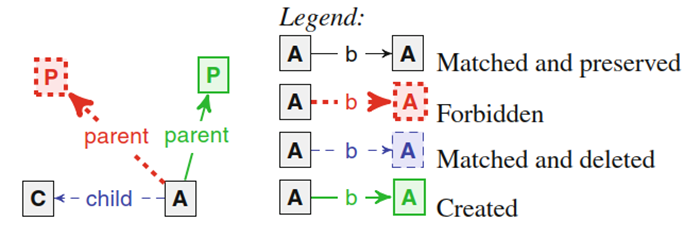
\includegraphics[width=11.03cm, height=4.0cm]{groove_legend}
\caption{Example GROOVE rule and legend  \cite{ghamarian2012modelling} }\label{fig:groove_legend}
\end{figure}
\begin{itemize}
\item The black (continuous thin) \enquote{reader} elements, in this case two nodes labelled \textbf{A} and \textbf{C}, must be present and are preserved—in fact, they form a positive application condition.
\item The \textcolor{red}{red} (dashed fat) \enquote{embargo} elements, in this case a \textbf{parent}-labelled edge with a \textbf{P}-labelled target node, must be absent in the graph—in fact, each connected subgraph of embargo elements forms a negative application condition.
\item The \textcolor{blue}{blue} (dashed thin) \enquote{eraser} elements, in this case a \textbf{child}-labelled edge from the \textbf{A}-node to the \textbf{C}-node, must be present and are deleted.
\item The \textcolor{green}{green} (continuous fat) \enquote{creator} elements, in this case a parent-labelled edge with a \textbf{P}-labelled target node, are created.
\end{itemize}
The overall effect of the rule is to search for \emph{\textbf{A}}- and \emph{\textbf{C}}-nodes connected by a \emph{\textbf{child}}-edge but without a \emph{\textbf{parent}}-edge to a \emph{\textbf{P}}-node, and to modify this by removing the \emph{\textbf{child}}-edge and adding a \emph{\textbf{parent}}-edge to a fresh \emph{\textbf{P}}-node.

 For instance, the rule can be applied to the graph on the left-hand side of Figure \ref{fig:groove_example}  in two ways, one of which result in the graph on the right-hand side. (The other application removes the other \emph{\textbf{child}}-edge.)

The core functionality of GROOVE is to recursively apply all rules from a predefined set (the graph transformation system) to a given start graph, and to all graphs generated by such applications. This results in a state space consisting of the generated graphs. The strategy according to which the state space is explored (\emph{e.g.}, depth-first, breadth-first or linear) can be set as a parameter \cite{ghamarian2012modelling}.
\begin{figure}
\center
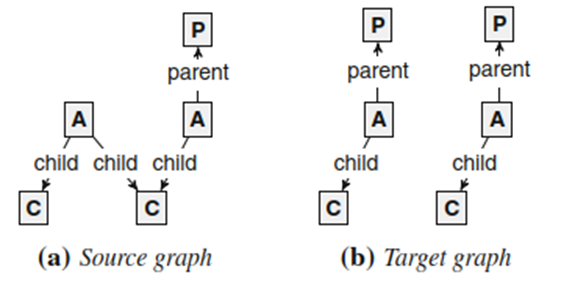
\includegraphics[width=9.73cm, height=4.79cm]{groove_example}
\caption{Example application of the rule in Figure \ref{fig:groove_legend}}\label{fig:groove_example}
\end{figure}\\ 
\textbf{Attributes}\\ 
Nodes in a graph typically stand for instances of some resource or concept. It is also necessary to include data fields, containing Booleans, integer numbers or strings. Such data fields are usually called \emph{attributes}. 

GROOVE supports attributes by treating them as special edges that do not point to a standard node, but to a node that corresponds to a data value. Graphically, such edges are usually represented by expressions of the form \enquote{x = 12}, rather than by x-labelled arrows pointing to a $12-labelled$ node.\\ 
\textbf{Regular expressions}\\
Besides ordinary edges, a rule may include edges carrying regular expressions. These will be matched in the host graph by searching for a path whose labels satisfy the regular expression. 

This especially allows the specification of cycles or the transitive closure of edges. Regular expressions may also contain \emph{wildcards}, which are matched by any label in a given set. Moreover, wildcard may be \emph{named}; such a name is effectively a variable for edge labels.\\ 
\textbf{Quantification}\\ 
One of the special features of GROOVE is the support of universal quantification in rules \cite{rensink2009repotting}. A universally quantified (sub)rule is one that will be applied to all subgraphs that satisfy the relevant application conditions, rather than just a single one as in the standard case. 

Such a rule can itself be much more concise, and also result in a smaller state space, then the equivalent set of rules that would ordinarily be needed. In fact, quantification can be nested in the sense that universally quantified rules can contain further existential subrules, and vice versa. Among other things, this makes it possible to formulate powerful application conditions \cite{rensink2004representing}.\\ 
\textbf{Control}\\ 
The standard behavior of GROOVE is to attempt the application of arbitrary rules at any point in time. There are, however, two further methods to control and direct the application of rules. A most straightforward mechanism is to assign \emph{priorities} to rules: low-priority rules may only be applied if no higher-priority rule is applicable. A more sophisticated mechanism is to use GROOVE’s \emph{control language}.
A control program is imposed on top of a graph transformation system and specifies the allowed order of application of the rules of that system, referring to the rules by name. 

For instance, the control program \emph{a}; try \{b;\} else \{c;\} specifies that first the rule named \enquote{a} must be applied, after which \enquote{b} is tried; if \enquote{b} is not applicable, \enquote{c} is applied. If rule \enquote{a} is not applicable in the beginning, then nothing happens. Other constructs offered by the language include:
\begin{itemize}
\item Looping, including an \enquote{as-long-as-possible} construct
\item A random choice between rules
\item Simple (noun-recursive) function calls
\end{itemize}
\textbf{State space exploration}\\ 
The most distinguishing feature of GROOVE, compared with another graph transformation tools, is the fact that it does not just carry out a single sequence of transformations from a given start state, but can explore and store the entire state space of reachable graphs. This provides a rich source of information for further analysis. In fact, GROOVE offers a choice of the exploration strategy to be used:
\begin{itemize}
\item Depth-first full exploration, also with on-the-fly Linear Temporal Logic model checking
\item Breadth-first full exploration. In some grammars, this enables finding shortest paths to certain graphs
\item Linear, random linear, and conditional exploration. This allows simulation without covering all states, for instance if the state space is too large.
\end{itemize}
In \cite{lucassen2016improving} Kleppe et al. describe the execution semantics of a simple object-oriented programming language in terms of graph transformation rules. A program graph is used as input and each rule application simulate the execution of a program instruction. By means of GROOVE’s state space exploration capabilities, it is possible to generate finite execution traces of a program and model check for errors. In this setting, GROOVE can be seen as a non-deterministic execution engine for the language defined by the transformation rules.

GROOVE can provide a great assistance in analyzing US, where non-determinism as well as parallelism is an essential part. However, the problem does not scale in GROOVE for problems with large sizes. This is because the size of the state space grows dramatically as the ring size increases. This is the well-known state space explosion problem, common to all model checking tools \cite{rensink2004representing}.
\begin{example}
To exemplify model checking in GROOVE, we consider a finite transition system consisting of two USs, $US_1$:\enquote{As an Administrator, I am able to add a new person to the database} and  $US_2$: \enquote{As a Visitor, I am able to view a person’s profile}. The application of typed graph and transformation rules, as depicted in Figure \ref{fig:groove_transformation_rules}, utilizing two transformation rules: one corresponds to $US_1$ named $add\_person$; it serves the purpose of saving a Profile in the database when there is no existing Profile (corresponding to specific Person in the database). Another rule corresponding to $US_2$ named $view\_profile$ is responsible for adding a \enquote{view} edge between Visitor and the DB nodes if a Profile (corresponding to the Person) already exists in the database. AS we can see both rules are typed according to defined type graph .As start graph we choose the existent of four Element namely Admin, DB, Visitor and Profile.
\begin{figure}
\center
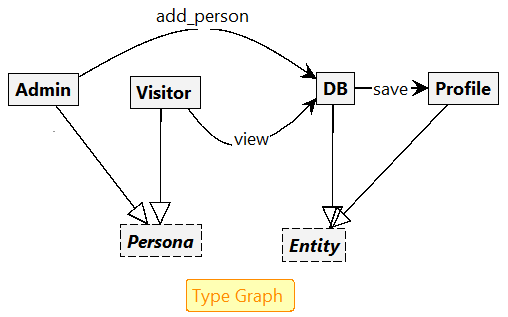
\includegraphics[height=7.5cm,width=13.3cm]{groove_typed_graph}
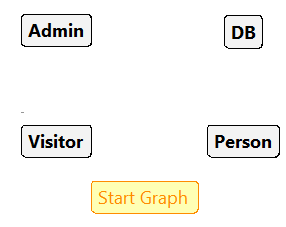
\includegraphics[height=4.5cm,width=5.3cm]{groove_start_graph}
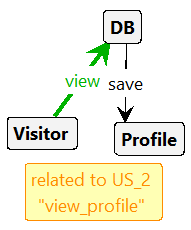
\includegraphics[height=5cm,width=5.43cm]{groove_rule_view_profile}
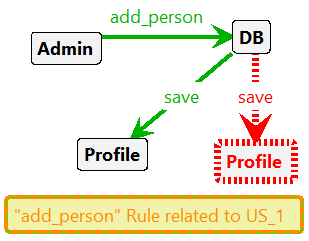
\includegraphics[height=5.5cm,width=8cm]{groove_rule_add_person}
\caption{Provided Type-Graph, Start Graph and Transformation Rules for $US_1$ and $US_2$ } \label{fig:groove_transformation_rules}
\end{figure}
\begin{figure}
\center
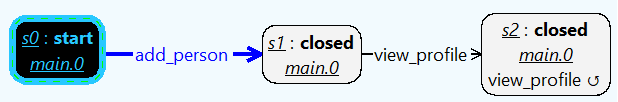
\includegraphics[width=14.0cm, height=2.3cm]{groove_model_checking}
\caption{Application of GROOVE model checking to Analyze Transformation Rules and a finite transition system for two USs }\label{fig:groove_model_checking}
\end{figure}
\end{example}
The application of GROOVE model checking to analyze transformation rules and a finite transition system is illustrated in Figure \ref{fig:groove_model_checking}. As we can see, GROOVE found only a single sequence of transformation, which means, $US_2$ cannot proceed without execution and consideration of $US_1$ due to lack of \textbf{save}-edge between \textbf{Profile}-node and \textbf{DB}-node. 

\subsection{Henshin: A Tools for In-Place EMF Model Transformations}\label{henshin}
The Eclipse Modelling Framework (EMF) provides modelling and code generation facilities for Java applications based on structured data models. Henshin is a language and associated tool set for in-place transformations of EMF models. 

The Henshin transformation language uses pattern-based rules on the lowest level, which can be structured into nested transformation units with well-defined operational semantics. So-called amalgamation units are a special type of transformation units that provide a forall-operator for pattern replacement. For all of these concepts, Henshin offers a visual syntax, sophisticated editing functionalities, execution and analysis tools. The Henshin transformation language has its roots in attributed graph transformations, which offer a formal foundation for validation of EMF model transformations \cite{arendt2010henshin}. \\ 
\textbf{Graph Types}\\ 
Graph transformation-based approaches, essentially define model transformations using rules consisting of a pre-condition graph, called the left-hand side (LHS), and a post-condition graph, called the right-hand side (RHS) of the rule. Informally, the execution of a model transformation requires that a matching of objects in the model (host graph) to the nodes and edges in the LHS is found, and these matched objects are changed in such a way that the nodes and edges of the RHS match these objects \cite{tichy2013detecting}.

The performance of graph transformation-based model transformations is mainly determined by the efficiency of the match finding of the LHS. Consequently, model transformation languages offer different options to add constraints to the LHS of model transformations to improve the performance of the matching \cite{tichy2013detecting}. To be efficient, graph transformation tools usually employ heuristics such as search plans to provide good performance (e.g. \cite{varro2012algorithm}).\\ 
\textbf{Structure and Application of Rules}\\ 
The Henshin transformation language is defined by means of a metamodel. The Henshin metamodel is closely aligned to the underlying formal model of double pushout (DPO) graph transformations \cite{tichy2013detecting}. Thus, rules consist of a left-hand side and a right-hand side graph as instances of the \emph{Graph} class. Rules further contain node mappings between the LHS and the RHS which are omitted here for better readability. Graphs consist of a set of Nodes and a set of Edges. Nodes can additionally contain a set of Attributes. These three kinds of model elements are typed by their corresponding concepts in the Ecore metamodel of EMF.\\ 
\textbf{Application Conditions}\\ 
To conveniently determine where a specified rule should be applied, application conditions can be defined. An important subset of application conditions is negative application conditions (NACs) which specify the non-existence of model patterns in certain contexts.
In the Henshin transformation model, graphs can be annotated with application conditions using a \emph{Formula}. This formula is either a logical expression or an application condition, which is an extension of the original graph structure by additional nodes and edges. A rule can be applied to a host graph only if all application conditions are fulfilled \cite{arendt2010henshin}.\\
\textbf{Attribute and Parameters}\\ 
Nodes may also include a set of Attributes. Rules inherit from Units and can thus include various Parameters. A common use of parameters is to transmit an Attribute value (such as a name) from a node to be matched in the rule. To restrict the application of a rule, the metamodel encompasses concepts for representing nested graph conditions \cite{habel2009correctness} as well as attribute conditions.\\ 
\textbf{State space exploration}\\ 
Henshin support in-place model transformation, Arendt et al. have developed a state space generation tool, which allow to simulating all possible executions of a transformation for a given input model, and to apply model checking, similar to the GROOVE \cite{kastenberg2006model} tool. Henshin can generate finite as well as large state space exploration. Regarding generation and analysis of large state space, the tool’s ability to utilize parallel algorithms, taking advantage of modern multi-core processors, which enables the handling of state spaces with millions of states. \\ 
\textbf{Analyzing Conflicts and Dependencies}\\ 
The elements that comprise the system under construction interact with each other, establishing dependencies among them \cite{kastenberg2006model}. In Figure \ref{fig:inherited_dependencies}, \emph{element A} requires \emph{element B}, generating a dependency between them. Such dependencies are naturally inherited by the user stories ($US_i$ 
cannot be implemented until $US_j$ is implemented). 

Therefore, the natural dependencies between USs should be accepted as inevitable. In fact, only a fifth of the requirements can be considered with no dependencies \cite{carlshamre2001industrial}. The existence of dependencies between USs makes it necessary to have some implemented before others \cite{carlshamre2001industrial},\cite{Greer2004},\cite{logue2008handling}. If the order of USs implementation does not consider these dependencies, it may have a large number of preventable refactorings, increasing the total cost of the project needlessly. Identifying beforehand the dependencies increases the ability to effectively deal with changes. 

Hence, light systematic mechanisms are needed to help identify dependencies between USs \cite{gomez2010systematic}.
\begin{figure}
\center
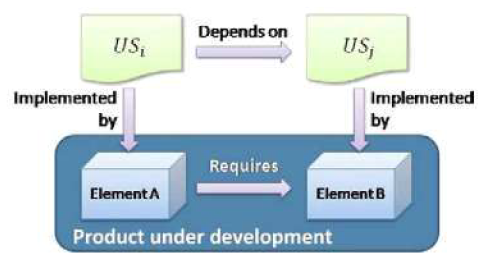
\includegraphics[width=12.03cm, height=6.7cm]{inherited_depencendy}
\caption{  Inherited dependencies by user stories\cite{gomez2010systematic} }\label{fig:inherited_dependencies}
\end{figure}
The critical pair analysis (CPA) for graph rewriting \cite{hartmanis2006monographs} has been adapted to rule-based model transformation, \emph{e.g.} to find conflicting functional requirements for software systems \cite{hausmann2002detection}, or to analyses potential causal dependencies between model refactorings \cite{mens2007analysing}, which helps to make informed decisions about the most appropriate refactoring to apply next. The CPA reports two different forms of potential causal dependencies, called conflicts and dependencies \cite{born2015analyzing}.
The application of a rule $r_1$ is in conflict with the application of a rule $r_2$ if
\begin{itemize}
\item[--] $r_1$ deletes a model element used by the application of $r_2$ \textbf{(delete/use)}, or
\item[--] $r_1$ produces a model element that $r_2$ forbids \textbf{(produce/forbid)}, or
\item[--] $r_1$ changes an attribute value used by $r_2$ \textbf{(change/use)}\footnote{Dependencies between rule applications can be characterized analogously.}. 
\end{itemize}
%The subsequent dependency results differ in their target of the second attribute movement. The first produce/use-dependency (2) represents the case of moving the attribute back to the original class, which leads to a smaller minimal model with only two classes referencing each other, as depicted in Figure \ref{fig:minimal_model}. The highlighting by enclosing hash marks is the most important information, since the enclosing element is the cause of the dependency. The link between 2:Class and 3:Attributeis created by the first rule application and is required by the second application. Since all elements and values in the minimal model may be matched by the first and the second rule application, there is a generic approach to represent attribute values. Value r1\_source\_r2\_target , \emph{e.g.}, means that it must conform to value source in rule $r_1$ and value target in rule  $r_2$ , respectively (compare Figure \ref{fig:henshin_refractoring_rule}(a)). The second dependency reported in Figure \ref{fig:cpa_result} is the handling of two consecutive attribute shifts \cite{mens2007analysing}.\\ 
\textbf{Different between Model Checking and Conflict and Dependency Analysis}\\ 
In this subsection, we shall delineate two distinct analytical methodologies, specifically model checking and Conflict and Dependency Analysis. Their respective purposes are delineated in Table \ref{tb:sec_6_comparative_analysis}, which serves to elucidate their appropriateness for modelling USs.

\begin{figure}
\begingroup
\footnotesize
\centering
\begin{tabularx}{\textwidth}{l  X  X}
\hline
Aspect	&Model Checking for User Stories &	Conflict and Dependency Analysis for User Stories \\
\hline\hline
Purpose	&Verify user story properties and system behavior	&Understand dependencies and interactions between user stories \\\\ 
Method&	Large state spaces exploration&	Rule-based model transformation\\\\ 
Automated vs. Manual&	Automated	&Automated\\\\ 
Scope&	Ensuring user stories meet specified requirements and system behavior	&Understanding how user stories relate to each other, managing dependencies\\\\ 
Use Cases&	Ensuring user story correctness and system behavior	&Agile development, impact analysis, and managing user story dependencies\\\\ 
Result	&Verification of user story properties (e.g., acceptance criteria)	&Identification of user story dependencies, potential conflicts, and their impact on the development process\\\\ 
\hline
\end{tabularx}
\begin{TableCaption}
\caption{Comparative analysis between model checking and conflict and dependency methods}\label{tb:sec_6_comparative_analysis}
\end{TableCaption}
\endgroup
\end{figure}
\begin{example}
Similar to the presented instance in GROOVE (as demonstrated in example \ref{groove_example}), we exemplify conflicts and dependencies within Henshin using identical user stories ($US_1$:\enquote{As an administrator, I can add a new person to the database} and $US_2$: \enquote{As a visitor, I can view a person's profile}). Figure \ref{fig:henshin_model} delineates the  class model LDAP (Lightweight Directory Access Protocol). In Figure \ref{fig:henshin_rule}, the defined rules in Henshin, specifically the rule view\_profile linked to $US_2$, and add\_person\_profile corresponding to $US_1$, are depicted. The representation uses black to signify object preservation and green for new objects. In addition, Figure \ref{henshin_cpa_result} (CDA result) shows the dependencies between $US_2$ and $US_1$ as \emph{\enquote{Create dependency}}, which highlights that \emph{Profile} node must first be created by $US_1$ in order to be used in $US_2$. Last but not least, a special instance graph is not required in Henshin.
\begin{figure}
\center
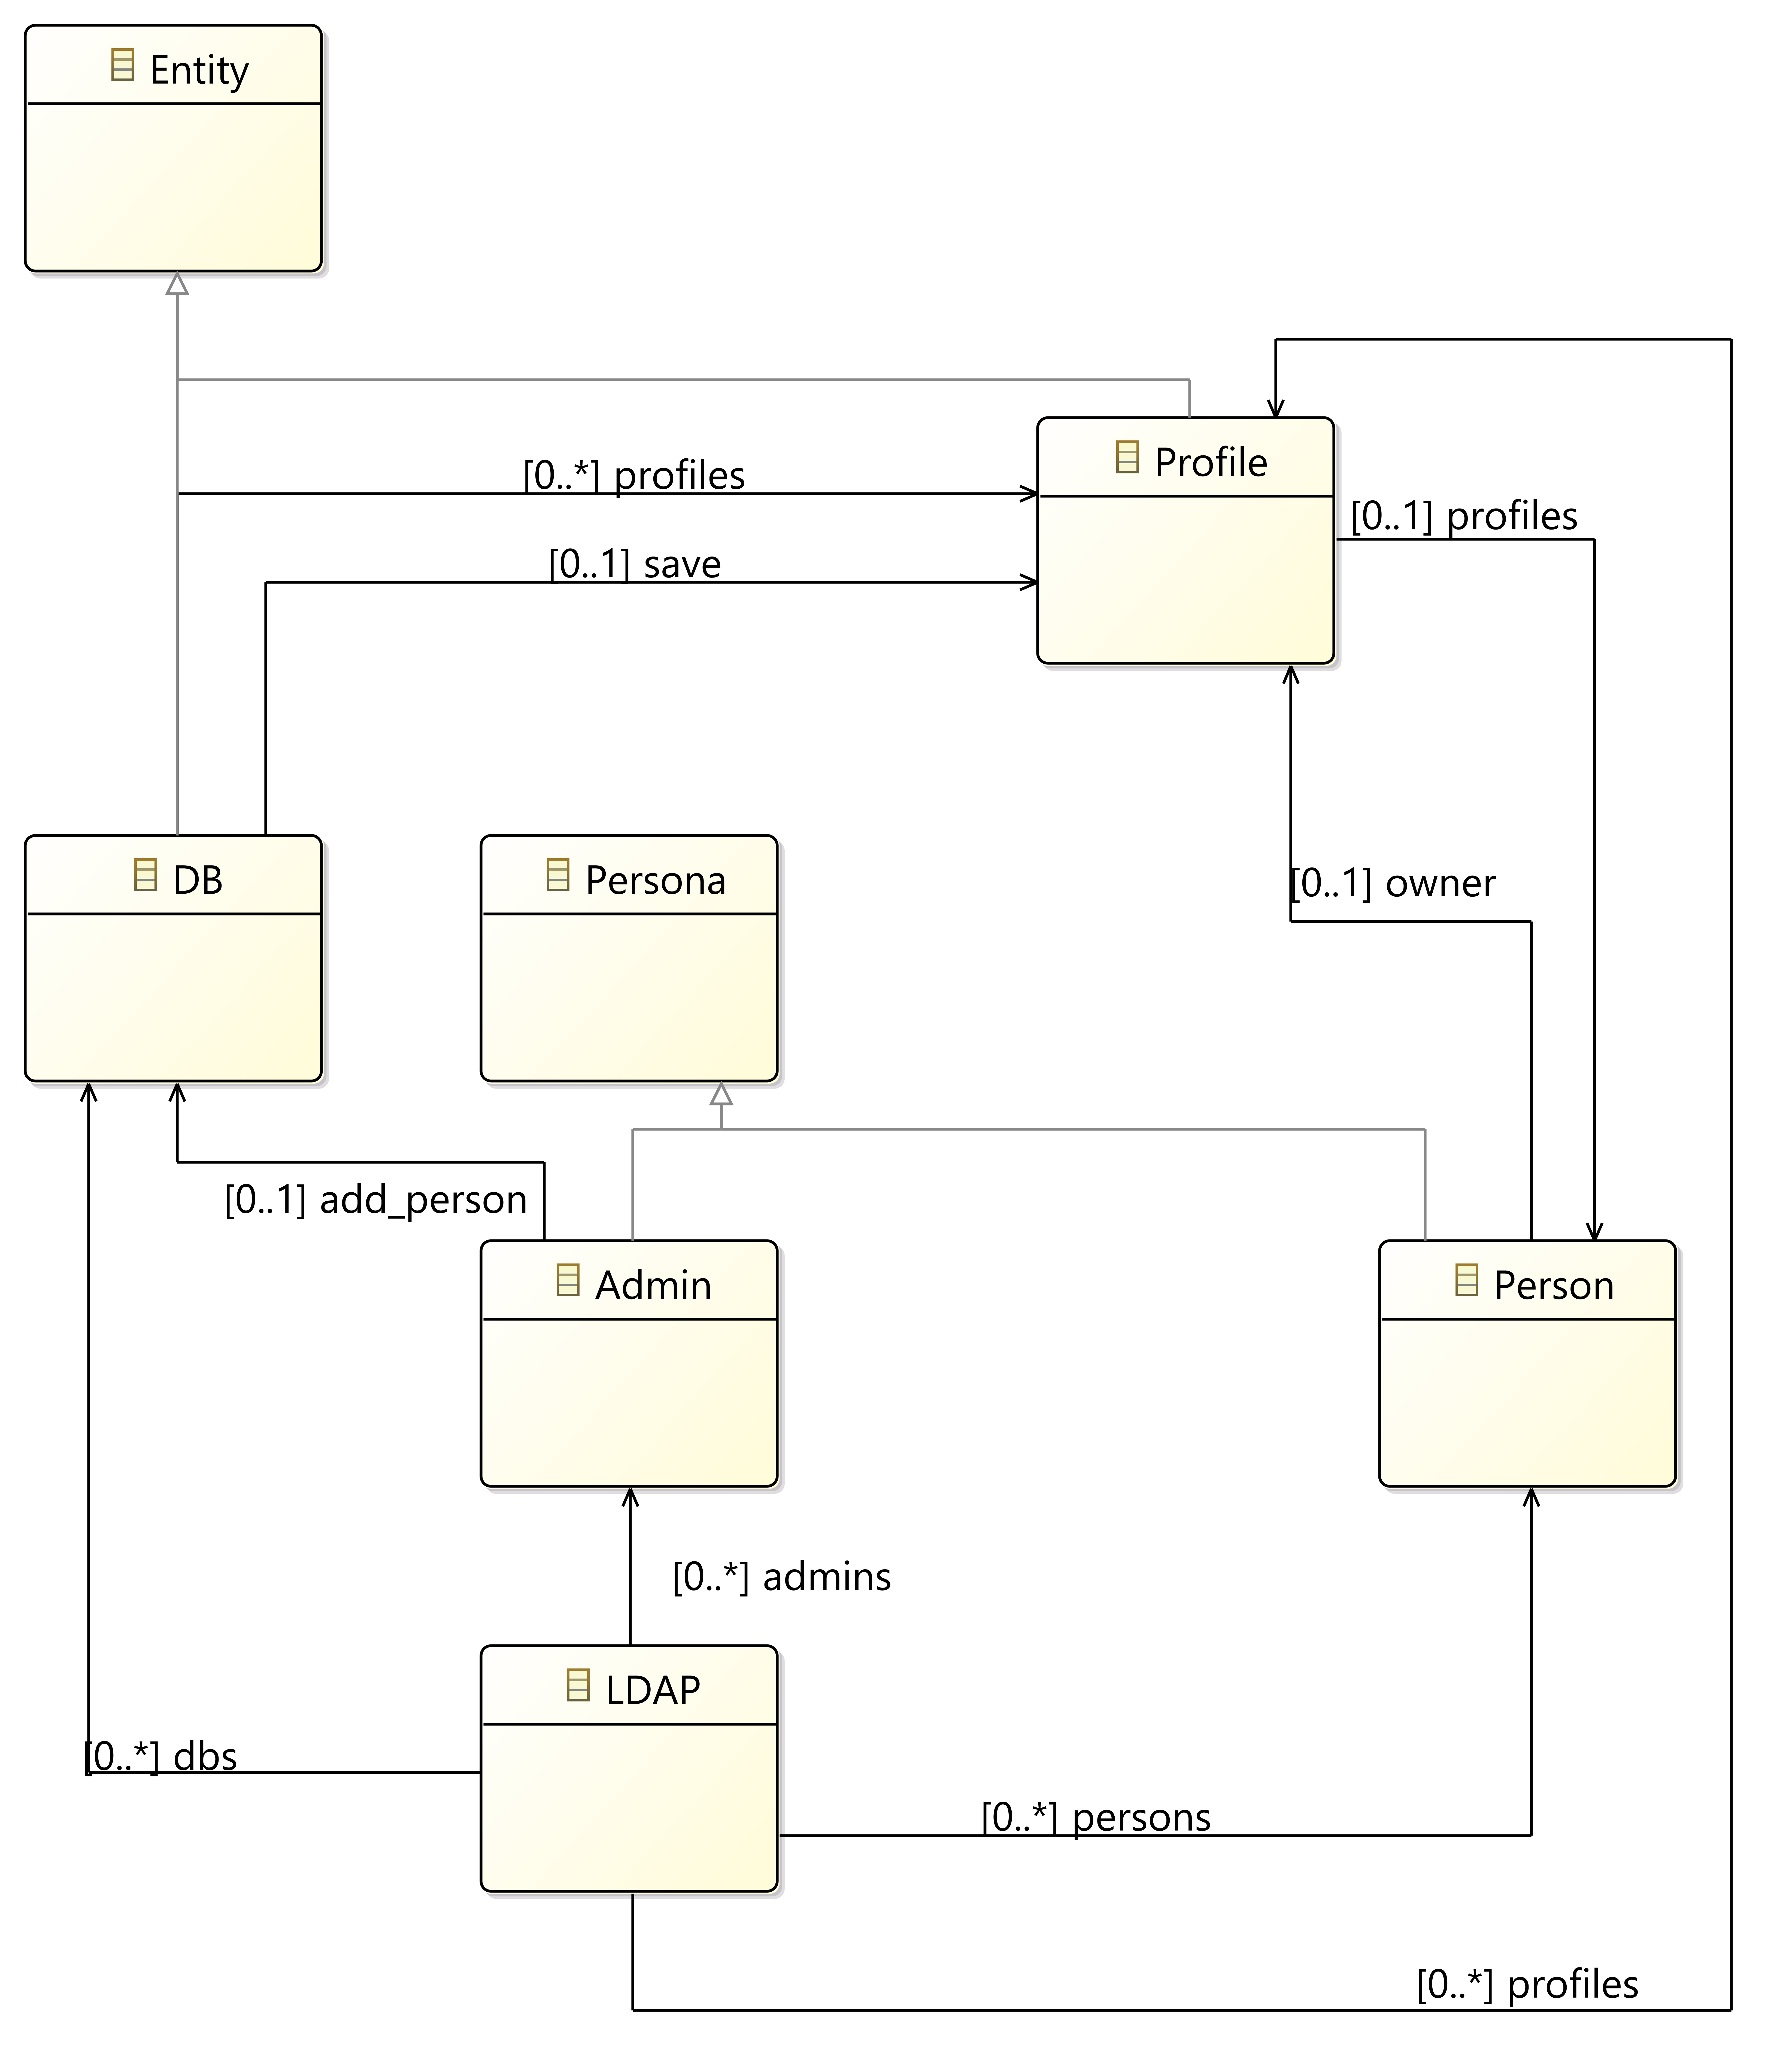
\includegraphics[width=13.13cm, height=13.6cm]{henshin_class_model}
\caption{Henshin Class Model LDAP}\label{fig:henshin_model}
\end{figure}
\begin{figure}
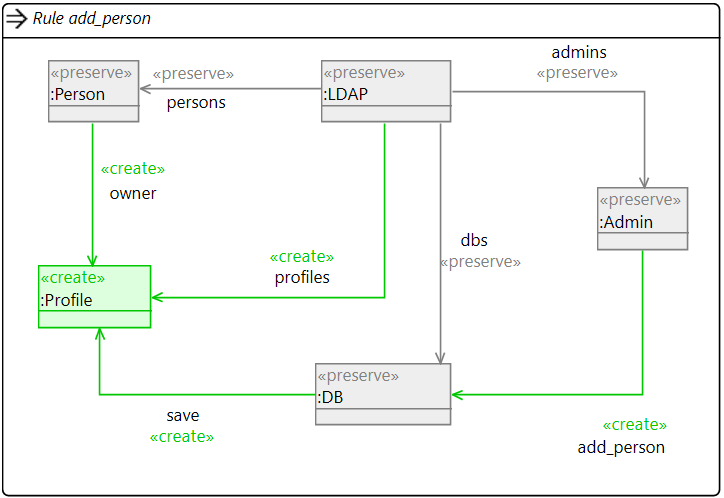
\includegraphics[width=13.13cm, height=7.6cm]{henshin_rule_add_person}
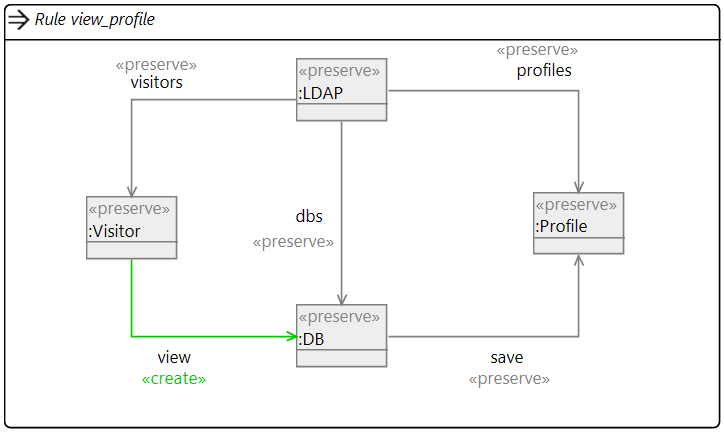
\includegraphics[width=13.13cm, height=7.6cm]{henshin_rule_view_profile}
\caption{Illustrated rules in Henshin: view\textunderscore{profile} rule related to $US_2$ and add\textunderscore{person} related to $US_1$}\label{fig:henshin_rule}
\end{figure}
\begin{figure}
\center
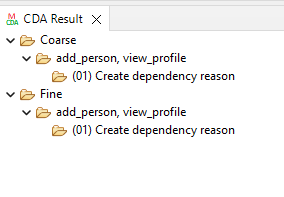
\includegraphics[width=8.13cm, height=5.6cm]{henshin_cpa_result}
%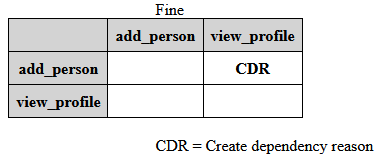
\includegraphics[width=8.13cm, height=3.6cm]{henshin_result}
\caption{Henshin CDA result visualises dependencies between user stories}\label{henshin_cpa_result}
\end{figure}
\end{example}
\begin{example}
Looking at the USs mentioned in the example \ref{example_conflict}, $US_1$: \enquote{As a user, I am able to edit any landmark.} and $US_2$:\enquote{As a user, I am able to delete only the landmarks that I added.}. First, we minimize $US_1$ and divided it into three USs as follows:
\begin{itemize}
\item $US_1a$:\enquote{As a user, I am able to add any landmark.}
\item $US_1b$:\enquote{As a user, I am able to modify any landmark.}
\item $US_1c$:\enquote{As a user, I am able to delete any landmark.}
\end{itemize}
Figure \ref{fig:conflict_model} shows the class model \enquote{Map} while figure \ref{fig:conflict_rule} shows the defined rules in Henshin, with each rule corresponding to a user story.

If $US_1c$ is translated into a rule and then CDA (Conflict and Dependency Analysis) is applied (Figure \ref{fig:conflict_cda}), Henshin would find a \enquote{Delete-Delete} conflict. This conflict can be avoided if $US_1c$ is replaced with $US_2$, as two users are then no longer allowed to delete the same landmark.

Figure \ref{fig:conflict_cda} shows the conflicts and dependencies either between two rules or between a rule and itself. For instance, there is a \enquote{Delete-Delete} conflict in $US_1c$. If the specific landmark are deleted, $US_1c$ cannot be applied anymore. 

Furthermore, there is a \enquote{Create-Delete} conflict between $US_1b$ and $US_2$. If the specific landmark are deleted, $US_1b$ cannot modify that landmark anymore.

The CDA is also able to recognise inconsistencies between user stories. The inconsistency for example between $US_1c$ and $US_2$ can be recognised because the corresponding rules also have a \enquote{Delete-Delete} conflict. This occurs when the same landmark is deleted. %However, we are investigating the extent to which inconsistencies can be recognised at all. That would be another open question.

\begin{figure}
\center
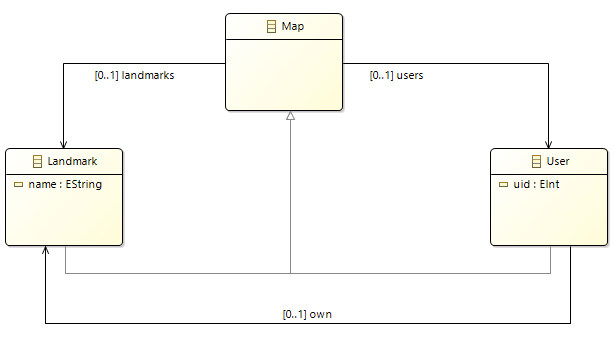
\includegraphics[width=8.28cm, height=7.6cm]{henshin_conflict_model}
\caption{Henshin Class Model Map}\label{fig:conflict_model}
\end{figure}
\begin{figure}
\center
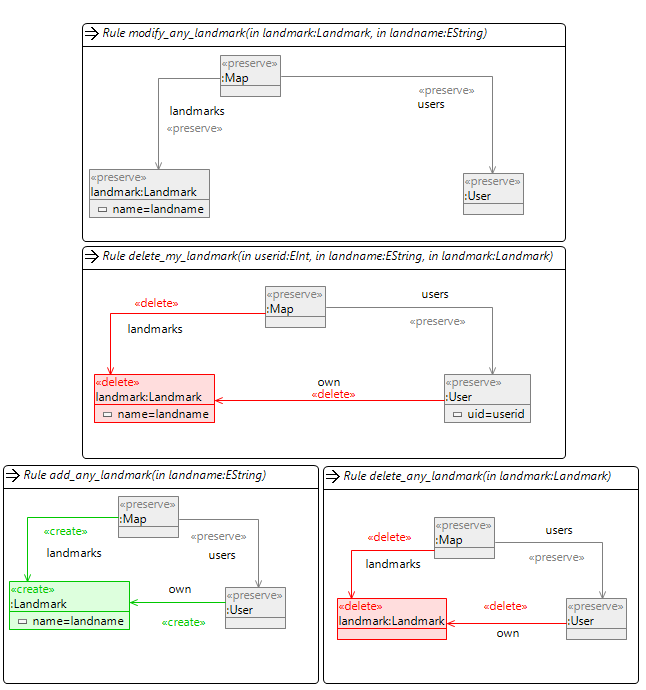
\includegraphics[width=13.13cm, height=10.6cm]{henshin_conflict_rule}
\caption{Illustrated rules in Henshin: add\textunderscore{landmark} rule related to $US_1a$, delete\textunderscore{any}\textunderscore{landmark} rule related to $US_1c$, modify\textunderscore{landmark} rule related to $US_1b$ and delete\textunderscore{my}\textunderscore{landmark} rule related to $US_2$ }\label{fig:conflict_rule}
\end{figure}
\begin{figure}
\center
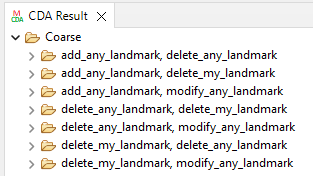
\includegraphics[width=9.2cm, height=9.9cm]{henshin_conflict_cda_result}
\caption{Henshin CPA result visualises conflicts and dependencies between user stories}\label{fig:conflict_cda}
\end{figure}
\end{example}

%\begin{example}
%To demonstrate the main idea of refactoring in Henshin Born et al. represent an example for class modeling limited to one rule \cite{born2016algorithm}. Rule \emph{Move\_Attribute} (Figure \ref{fig:henshin_refractoring_rule} (a)) specifies the shift of an attribute from its owning class to an associated one along a reference. It is shown in abstract syntax. Objects and references tagged by \emph{\texttt{<<preserve>>}} represent unchanged model elements, elements tagged by \emph{\texttt{<<create>>}} represent new ones whereas those tagged by \emph{\texttt{<<delete>>}} are removed by the transformation \cite{mens2007analysing}.


%\begin{figure}
%\center
%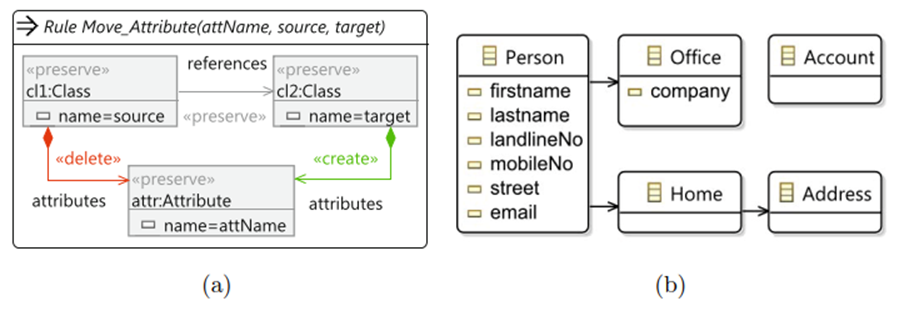
\includegraphics[width=14.13cm, height=5.0cm]{Henshin_refactoring_rule }
%\caption{Henshin refactoring rule (a) and class model Address Book (b) \cite{mens2007analysing} }\label{fig:henshin_refractoring_rule}
%\end{figure}
%Modifying the class model in Figure \ref{fig:henshin_refractoring_rule}(b) by the refactoring specified in Figure \ref{fig:henshin_refractoring_rule}(a), Born et al. observe two potential problems: (1) the attribute \emph{landlineNo} of class Person can be shifted to either class Home or class \emph{Office} (by refactoring\emph{ Move\_Attribute}) \cite{mens2007analysing}. However, if it is shifted to class Home the other refactoring becomes inapplicable (and vice versa). This means, refactoring \emph{Move\_Attribute} is in conflict with itself. (2) The attribute street of class \emph{Person} can be shifted to class \emph{Address} via class \emph{Home} (by two applications of\emph{ Move\_Attribute} along existing references). The second shift is currently not possible since class \emph{Home} does not have an attribute so far, i.e., refactoring Move\_Attribute may depend on itself. Graph transformation theory allows us to analyze such conflicts and dependencies at specification time by relying on the idea of the CPA \cite{mens2007analysing}.
%\end{example}
\textbf{CPA Tool}\\
The provided CPA extension of Henshin can be used in two different ways: Its application programming interface (API) can be used to integrate the CPA into other tools and a user interface (UI) is provided supporting domain experts in developing rules by using the CPA interactively \cite{mens2007analysing}.

After invoking the analysis, the rule set and the kind of critical pairs to be analyzed have to be specified. Furthermore, options can be customized to stop the calculation after finding a first critical pair, to ignore critical pairs of the same rules, etc. The resulting list of critical pairs is shown and ordered along rule pairs. 

%Figure \ref{fig:cpa_result} depicts an example for the analysis of rule \emph{Move\_Attribute}, in which the\emph{ delete/use conflict} (1) corresponds to the example illustrated in figure \ref{fig:minimal_model} \cite{mens2007analysing}.
%The subsequent dependency results differ in their target of the second attribute movement. The first produce/use-dependency (2) represents the case of moving the attribute back to the original class, which leads to a smaller minimal model with only two classes referencing each other, as depicted in Figure \ref{fig:minimal_model}. The highlighting by enclosing hash marks is the
%most important information, since the enclosing element is the cause of the dependency. The link between 2:Class and 3:Attribute is created by the first rule application and is required by the second application. Since all elements and values in the minimal model may be matched by the first and the second rule application, there is a generic approach to represent attribute
%values. Value \emph{r1\_source\_r2\_target}, e.g., means that it must conform to value source in rule \emph{r1} and value target in rule \emph{r2}, respectively (compare Fig. \ref{fig:henshin_refractoring_rule}(a)).

%The second dependency reported in Figure \ref{fig:cpa_result} is the handling of two consecutive attribute shifts.

%\begin{figure}
%\center
%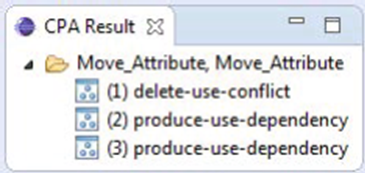
\includegraphics[width=6.22cm, height=2.96cm]{cpa_result}
%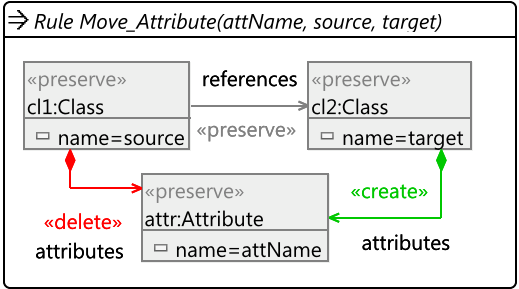
\includegraphics[width=6.22cm, height=2.96cm]{rule_move_attribute}
%\caption{The result view\cite{born2015analyzing} }\label{fig:cpa_result}
%\end{figure}
%\begin{figure}
%\center
%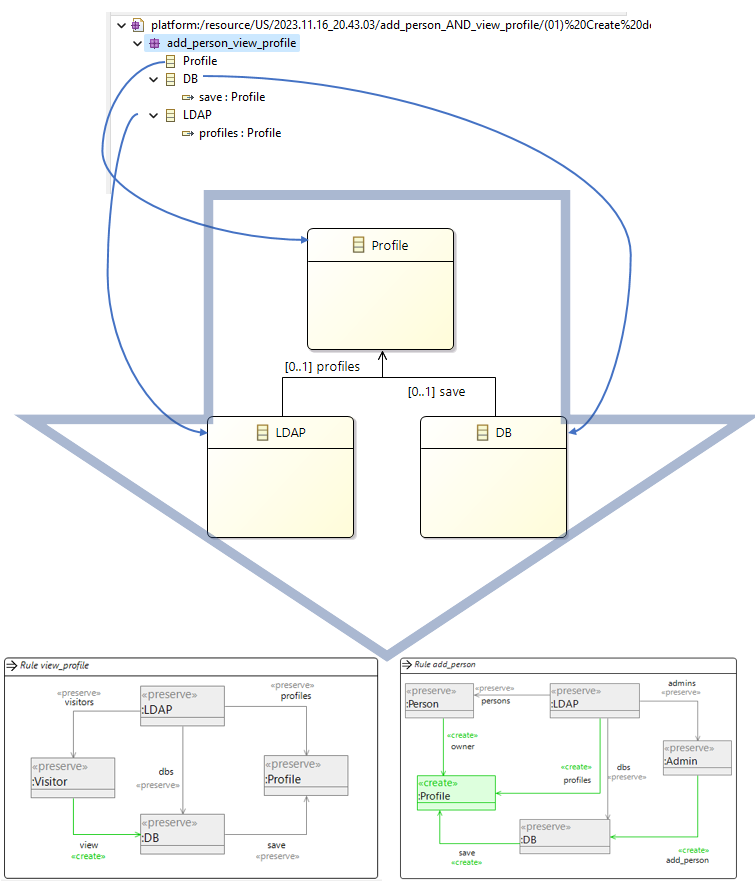
\includegraphics[width=12.13cm, height=13.0cm]{detailed_representation}
%\caption{Detailed representation of a critical pair showing a dependency \cite{born2015analyzing} }\label{fig:minimal_model}
%\end{figure}

\subsection{Comparative Analysis}\label{sec_6_comparative_analysis}
In the following, we compare two graph-based modelling tools using different categories, inspired by \cite{ghamarian2012modelling}. 
\begin{itemize}
\item Area: Which Area does the tools support?
\item Typing: What is the typing mode that the tools operate in?
\item Control: How do the tools provide control over the application of rules?
\item Strategy: What strategies do the tools employ for analysis and conflict resolution?
\item Relevant Features: What advanced features and capabilities do the tools offer?
\item Interface: How user-friendly are the tools' interfaces?
\end{itemize}
An overview of this comparison is given in table \ref{tb:sec_6_comparative_analysis_final}. Finally, we choose one of these tools for our approach, namely analysis of conflicts and dependencies between user stories.

\begin{figure}
\begingroup
\footnotesize
\centering
\begin{tabularx}{\textwidth}{l  X  X}
\hline
Aspects&	GROOVE	&Henshin\\
\hline\hline
Area	&Model Transformation, Verification, Analysis, Simulation	&EMF-Based Transformation model, Analysis, Simulation, Verification \\ \\ 
Typing and Inheritance&	Node Types, Multiple Inheritance	&Multiple Inheritance\\\\ 
Control&	Rule Priorities, Control Program	&Non-Deterministic Rule Choices, Sequential and Priorities Over Transformation Unit \\\\ 
Verification&	 Full State Space Exploration, Model Checking	&Model Transformation System (Transformation Module) and Conflict Detection, State Space Exploration, Model Checking\\\\ 
Relevant Features&	Quantified Rules, Wildcards and Regular Expressions	&CPA Extension of Henshin\\\\ 
Interface&	GUI Helps Debugging, Prototyping, Analysis of Results	&GUI Helps Prototyping, GUI Helps Analysis of Results\\\\ 
Strong Points&	Rapid Prototyping, Local Confluence Check, Analysis Capabilities (only available at the state level, but not at the rule level as in Henshin), Rule Expressiveness	&Rapid Prototyping, Supporting Analyzing of Conflicts and Dependencies, Interoperability using API, Scalability, Performance\\\\ 
Weak Points&	Model Transformation Support, Interoperability, Scalability, Performance, Animation, Analyzing Conflicts and Dependencies 	&Required learning curve for new users to EMF and Transformation Process, Complexity in rule sequencing, Not support untyped mode\\\\ 
\hline

\end{tabularx}
\begin{TableCaption}
\caption{Overview of graph-based modelling tools inspired by \cite{ghamarian2012modelling}}\label{tb:sec_6_comparative_analysis_final}
\end{TableCaption}
\endgroup
\end{figure}
As a result of the introduction of the robust CPA (critical pair analysis) extension within the Henshin framework, our choice has shifted towards adopting Henshin over GROOVE. This strategic decision is underpinned by the unique capabilities of the CPA extension, which empower us to comprehensively evaluate conflicts and dependencies within graph-based transformation rules associated with USs. 

Moreover, a compelling factor in favor of Henshin is the inherent support of a versatile Application Programming Interface (API) by the CPA extension, facilitating seamless integration of CPA functionality into various tools, including Java-based platforms.

\subsection{Conclusion}\label{henshin_groove_conclusion}
It is imperative to note that Groove conducts its analysis with regard to particular instance graphs, whereas Henshin's (critical pair analysis (CPA) remains agnostic to the specifics of instance graphs. Consequently, model checking in Groove necessitates the entire state space, whereas Henshin merely requires the set of rules. In the Henshin approach, instance graphs are not explicitly selected; instead, only rule pairs are analysed, considering conflicts and dependencies. Usually, the state space in such systems becomes infinitely large, which is a challenge for GROOVE.

Since Henshin enables the specification of constraints and conditions within rules, which can be useful for enforcing and verifying US requirements to ensure that constraints are met.

In the Groove approach, it is not clearly defined what dependencies and conflicts mean. In the case of dependencies, the order in which rules are applied is specified, and this order is expected to be maintained in the state space. If there is no alternative order, it can be concluded that there is a dependency between the rules. Conflicts are similar: if rules can be applied in a graph and the resulting transitions are compatible with each other, there is no conflict. However, if the transitions are incompatible, there is a conflict. However, the analysis of the state space always depends on the instance graph selected at the beginning.



\section{Conclusion}\label{conclusion}
In Section \ref{usq}, we have undertaken a comparative analysis of various techniques for evaluating the quality of user stories, categorized according to different criteria. The INVEST criteria are deemed applicable in manual environments, such as those overseen by Product Owners, and necessitate a manual assessment against these criteria. The QUS framework, on the other hand, has been implemented through a tool named AQUSA to automate the process of assessing the quality of user stories. In our workflow's initial phase, we employ the QUS framework and AQUSA as tools to scrutinize user stories within the backlog, ensuring their applicability and alignment for subsequent actions.

In Section \ref{dmodel}, we conducted an experiment to assess the performance of the Visual Narrator, GPT-3.5, and CRF-based approach in automating the extraction of domain concepts from agile product backlogs. Given that the CRF generates a graph-based model, it is particularly advantageous for our approach, serving as input for the development of a transformation rule system.

Section \ref{nlp} revolves around the comparison of various lexical resource techniques for computation. VerbNet, specializing in verbs, FrameNet, with a broader spectrum encompassing nouns and adjectives, and WordNet, offering a wide array of words spanning various parts of speech, have been evaluated. 

For our purposes, VerbNet stands out as the most suitable technique. Its hierarchical classification of verbs into classes provides a structured and comprehensive approach for categorizing a wide range of verbs based on their semantics. This is of utmost importance in our endeavor to formulate transformation rules rooted in semantic interpretations of actions within user stories.

Finally, in Section \ref{gts}, we scrutinize graph transformation tools, specifically Henshin and GROOVE. GROOVE is best suited for comprehensive analysis of the full state space and random-linear exploration, proving highly effective for analytical and verification purposes. Henshin, on the other hand, is an EMF-based transformation model boasting scalability and interoperability as its key attributes. 

Notably, Henshin supports the analysis of conflicts and dependencies using the CPA extension. Furthermore, a persuasive attribute in favor of Henshin lies in its intrinsic provision of a versatile Application Programming Interface (API) through the CPA extension.

Owing to the utilization of various tools and techniques for ascertaining dependencies and conflicts among user stories, several pertinent questions arise: Can we succeed in classifying all verbs in roughly into three categories namely \enquote{create}, \enquote{delete} and \enquote{forbid}? With regard to the quality analysis presented, there are not suitable analyses for all criteria, what could the analysis for missing criteria look like? Can we use graph transformations to find conflicts and dependencies between annotated user stories? To what extent does the effectiveness of our approach hinge on the datasets provided within the backlogs? would we characterize the overall effectiveness of our approach? 





\newpage

\bibliographystyle{abbrv}
\bibliography{Literatur.bib}

   
\end{document}
